\documentclass[USenglish,phd]{uit-thesis}
\usepackage[inline]{enumitem}
\usepackage{bibentry}
\nobibliography*

\usepackage[acronym]{glossaries}
\usepackage{afterpage}

\makeglossaries

\newacronym{cwl}{CWL}{Common Workflow Language}
\newacronym{nowac}{NOWAC}{Norwegian Women and Cancer}
\newacronym{mixt}{MIxT}{Matched Interactions Across Tissues}
\newacronym{sr}{SR}{Systemic Response}
\newacronym{gatk}{GATK}{Genome Analysis Toolkit}
\newacronym{cran}{CRAN}{Comprehensive R Archive Network}
\newacronym{ide}{IDE}{integrated development environment}
\newacronym[plural=VMs, firstplural=Virtual Machines (VMs)]{vm}{VM}{Virtual Machine}
\newacronym{gpu}{GPU}{graphical processing unit}
\newacronym{dna}{DNA}{Deoxyribonucleic acid} 
\newacronym{rna}{RNA}{Ribonucleic acid} 
\newacronym{wes}{WES}{whole-exome sequencing}
\newacronym{wgs}{WGS}{whole-genome sequencing}
\newacronym{hts}{HTS}{High-throughput Sequencing} 
\newacronym{ngs}{NGS}{Next-generation Sequencing} 
\newacronym[plural=SNPs, firstplural=Single Nucleotide Polymorphisms (SNPs)]{snp}{SNP}{Single Nucleotide Polymorphism}
\newacronym[plural=GUIs, firstplural=graphical user interfaces (GUIs)]{gui}{GUI}{Graphical User Interface}
\newacronym{pfs}{PFS}{Pachyderm File System}
\newacronym{pps}{PPS}{Pachyderm Processing System}
\newacronym{xml}{XML}{Extensible Markup Language}
\newacronym{json}{JSON}{JavaScript Object Notation}
\newacronym{yaml}{YAML}{YAML Ain't Markup Language}
\newacronym{dag}{DAG}{directed acyclic graph}
\newacronym{hpc}{HPC}{High-Performance Computing}
\newacronym{wdl}{WDL}{Workflow Definition Language}
\newacronym{dsl}{DSL}{Domain Specific Language}
\newacronym{api}{API}{Application Programming Interface} 
\newacronym{csv}{CSV}{comma-separated values}
\newacronym[plural=GBs, firstplural=Gigabytes (GBs)]{gb}{GB}{Gigabyte} 
\newacronym{cli}{CLI}{Command-line Interface}
\newacronym{scm}{SCM}{source code management}
\newacronym[plural=SMEs,firstplural={Small Modular Entities (SMEs)}]{sme}{SME}{Small Modular Entity}
\newacronym[plural=GBs, firstplural=gigabytes (GBs)]{GB}{GB}{Gigabyte}
\newacronym{kegg}{KEGG}{Kyoto Encyclopedia of Genes and Genomes}


\begin{document} 

\title{Toward Reproducible Analysis and Exploration of High-Throughput
Biological Datasets}
\author{Bjørn Fjukstad}
\thesisprogramme{A dissertation for the degree of Philosophiae Doctor -- 2018}
\thesisfaculty{Faculty of Science and Technology \\ Department of Computer
Science}

\ThesisRightFrontpageImage{"figures/frntpg"}
\ThesisLeftFrontpageImage{"figures/frntpg"}

\maketitle

\frontmatter

\begin{epigraph}
\epigraphitem{Ta aldri problemene på forskudd, for da får du dem to ganger, men
    ta gjerne seieren på forskudd, for hvis ikke er det altfor sjelden du får
    oppleve den.}{Ivar Tollefsen}
\end{epigraph}

\begin{abstract}
    There is a rapid growth in the number of available biological datasets due
    to the decreasing cost of collecting and storing the data, together with
    high-throughput data collection instruments. Modern instruments enables
    analysis of biological data at different levels, from DNA sequences
    through cell structures and up to the function of organs. This leads to the
    potential for novel insights to the underlying biological mechanisms in the
    development and progression of diseases such as cancer. The wide range of
    these different biological datasets has led to the development of a wealth
    of software packages and systems for researchers to use in data exploration
    and analysis.

    Researchers tailor the exploration and analysis of their datasets using a
    range of different tools and systems. Because of the specialized nature of
    each step of the analysis, few of the tools provide useful interfaces for
    analyses across programming languages and frameworks. In addition, reporting
    the details of an analysis becomes a tedious task because of the long list
    of different tools, input parameters and reference to databases. The lack of
    such details can complicate reusing the analyses for other datasets, or even
    reproducing the results of the original data. This increases both analysis
    time and leaves unrealized potential for scientific insights.

    This dissertation argues that, instead, we can design systems for
    exploring and analyzing high-throughput biological datasets from small
    composable pieces. In particular we show the viability through software
    container technologies together with well-defined interfaces, configuration,
    and orchestration. This approach simplifies the development of analysis
    pipelines and interactive data exploration applications. In addition it
    provides the necessary information to reproduce analyses and share the
    methods across teams. 
    
    We show the feasibility of our approach through applications for analyzing
    high-throughput \gls{dna} sequencing datasets, and exploring gene expression
    data integrated with questionnaire, registry, and online databases. Our
    evaluation shows how we effectively capture provenance in analysis pipelines
    and exploration applications to simplify reproducibility and encourage
    sharing of methods and tools.
    
\end{abstract}

 
\begin{acknowledgement}
    First I would like to thank my advisor, Professor Lars Ailo Bongo for his
    relentless support and encouragement during my time as a PhD student. He has
    indeed shown me what tough love is, and I am grateful for that. 

    I would like to thank my co-advisors Professor Eiliv Lund and Associate
    Professor Karia Standahl Olsen for their wonderful ideas and warm welcome
    into a research field that was not my own. 

    I would like to extend my gratitude to Professor Michael Hallett and Vanessa
    Dumeaux for their hospitality when I visited their lab in Montreal in
    2016. I do not think this thesis would have been as interesting without the
    projects I was fortunate enough to be a part of. Thank you! 

    I would like to thank my long time office wife Einar, Morten, Nina, and
    the BDPS lab at UiT. 

    Thank you to past or current students at UiT: Jan-Ove, Vegard, Helge,
    Magnus, Erlend, Kristian, Martin, Amund, Michael, and many more. You have
    all contributed to nine wonderful years at the University!
    
    I would like to thank my colleagues at the Department of Computer Science,
    especially the technical staff, led by Maria Wulff Hauglann.
    %Also, the administrative staff at our School lab for
    %their wonderful collaborations. 
    
    Thank you to everyone in the \gls{nowac} research group, you have all been
    wonderful to collaborate with! 

    Thank you to the PhD students at Nordlandssykehuset in Bodø who have been my
    closest colleagues during the final push of my PhD. 
    
    I would like to thank my mom and dad, and my younger brother for their
    ever-present support. 

    Finally, Ane for her continuous love and support, and her
    \emph{endurance} through all of my big or small projects. 
\end{acknowledgement}
 

\tableofcontents

\printglossary[type=\acronymtype]

%\listofdefinition
\mainmatter


\chapter{Introduction}

% Thesis project two parts: 
% 1: Systems for exploring genomic data. Advanced statistical analyses from the
% web-browser or any other platform. 
% 2:  Analysis pipelines for large genomic datasets. Provenance of data. 
% 
% Common: 
% - Containers
% - Reproducibility
%     - 1: An application is an R package with the analyses. Do not need to
%     pre-compute results, can call functions etc. directly from the app. Build an
%     app as containers that can be shared. 
%     - 2: An analysis is a list of tools with 
%     input/output data. We package each tool in a container (snapshot-ish) 

\emph{Observation}:
Collecting large biological datasets have never been simpler
or cheaper. Data generation is growing at an unprecedented rate. There are a
wealth of software packages and systems to analyze these datasets, but they
often target only a small portion of the full analysis pipeline from raw data to
interpretable results.

\emph{Challenges}:
\begin{enumerate*}[label=(\roman*)]
    \item Giving a fully transparent overview of the data transformations from
        raw data to interpretable results; 
    \item Sharing an analysis pipeline across software platforms and research
        groups; 
    \item Providing full provenance of data, tools, and tool parameters; 
    \item Develop end-user applications that interface with the advanced
        statistical analyses required to explore biological datasets.  
    
\end{enumerate*} 

\emph{Related work}:
There are a wealth of related work and systems. To build analysis pipelines we
have systems such as
\begin{enumerate*}[label=(\roman*)]
    \item CWL and its implementations: cwl\_runner, Arvados, Rabix, Toil, Galaxy,
        AWE; and 
    \item Pahchyderm. 
\end{enumerate*}
When the data is analyzed and ready for further exploration, we have systems
such as
\begin{enumerate*}[label=(\roman*)]
    \item OpenCPU;
    \item RStudio and Shiny; 
    \item Renjin an R interpreter built on top of the JVM. 
\end{enumerate*}
 

\emph{Our solution}: 
To provide fully transparent overview of the statistical analyses from raw data
to interpretable results we propose our tool \emph{walrus}. It lets users create
and run analysis pipelines in bioinformatics to e.g. analyze high-throughput
sequencing datasets. In addition, it tracks full provenance of the input,
intermediate, and output data, as well as tool parameters. With \emph{walrus} we
have successfully built analysis pipelines to detect somatic mutations in breast
cancer patients. 

To develop applications that interface with the underlying statistical analyses
we have built \emph{Kvik}. Kvik allows applications written in any modern
programming language to interface with the wealth of bioinformatics packages in
the R programming language, as well as information available through online
databases. We have used Kvik to develop the MIxT system for exploring and
comparing transcriptional profiles from blood and tumor samples in breast cancer
patients. 

\emph{Advantages of our solution}:
Our analysis solution has the benefit that it integrates with modern version
control systems to provide provenance information on datasets. It also runs on a
wide range of software platforms and is targeted to the compute infrastructure
found in hospital environment. 

Our solution to build data explorations provides the benefit of developers being
able to develop applications in any programming language. It also facilitates
the reuse and interface with the wealth of statistical packages directly from a
user-interface rather than analysis scripts. 

\emph{Methods}:
% Litt usikker her LA? 

\emph{Long term contributions}:
Discuss why our approach works out nicely? Benefit for future use? Clinical
apps? 

\emph{Thesis statement}:
% Denne må jeg ha hjelp med! :) 
A hollistic approach to data analysis and exploration of high-throughput
dataasets in bioinformatics??? 

% alle stegene: pre-proessering, analyser, vise apps 
% hovedresultat: kapt 2
% exp: bcb-paperet 
% pipppelin epaper

\section{List of papers} 
\begin{itemize}
    \item
        \emph{Kvik: three-tier data exploration tools for flexible analysis of
        genomic data in epidemiological studies}
        \\
        \textbf{Bjørn Fjukstad}, Karina Standahl Olsen, Mie Jareid, Eiliv Lund,
        Lars Ailo Bongo. 
        \\ 
        F1000Research 2015.
        
    \item 
        \emph{Building Applications For Interactive Data Exploration In Systems
        Biology.}
        \\
        \textbf{Bjørn Fjukstad}, Vanessa Dumeaux, Karina Standahl Olsen, Michael
        Hallett, Eiliv Lund, Lars Ailo Bongo.  
        \\ 
        The 8th ACM Conference on Bioinformatics, Computational Biology, and
        Health Informatics (ACM BCB) 2017.

    \item 
        \emph{Interactions between the tumor and the blood systemic response of
        breast cancer patients.}
        \\ 
        Vanessa Dumeaux, \textbf{Bjørn Fjukstad}, Hans E Fjosne, Jan-Ole
        Frantzen, Marit Muri Holmen, Enno Rodegerdts, Ellen Schlichting,
        Anne-Lise Børresen-Dale, Lars Ailo Bongo, Eiliv Lund, Michael Hallett.
        \\ 
        PLoS Computational Biology 2017.

    \item \emph{A Review of Scalable Bioinformatics Pipelines} 
        \\
        \textbf{Bjørn Fjukstad}, Lars Ailo Bongo.
        \\ 
        Data Science and Engineering 2017.

    \item \emph{Reproducible Data Analysis Pipelines in Precision Medicine}
        \\
        \textbf{Bjørn Fjukstad}, Vanessa Dumeaux, Michael Hallett, Lars Ailo
        Bongo
        \\
        Conference TBA 2018. 


    \item \emph{nsroot: Minimalist Process Isolation Tool Implemented With Linux
        Namespaces.}
        \\
        Inge Alexander Raknes, \textbf{Bjørn Fjukstad}, Lars Ailo Bongo 
        \\
        NIK 2017. 
        
\end{itemize} 



 
From the discovery of the \gls{dna} structure by Watson and Crick in
1953\cite{watson1953molecular} to the sequencing of the human genome in 2001
\cite{venter2001sequence,international2001initial} and the massively parallel
sequencing platforms in the later years[6], the scientific advances have been
tremendous. Today, single week-long sequencing runs can produce as much data as
did entire genome centers just years ago.\cite{kahn2011future}  These
technologies allow researchers to collect data faster, cheaper and more
efficient, now making it possible to collect the entire genome from a patient in
less than a days work.

In this chapter we give a background in the different aspects of analyzing and
exploring biological datasets. We use the \gls{nowac} study as an example and
highlight the necessary processing steps from data generation and to
interpretation of results. In addition we describe the traditional data analysis
and management, and propose a novel approach for organizing, sharing, and
collaborating on research data and analyses. In this chapter we focus on
analysts writing their own specialized analysis scripts in programming languages
such as R. 

\section{High-Throughput Datasets in Research and Medicine} 
\gls{dna} sequencing is the process of determining the order of nucleotides
within a strand of \gls{dna}. 

Precision medicine uses patient-specific molecular information to diagnose and
categorize disease to tailor treatment to improve health
outcome.\cite{national2011toward} Important research goal in precision medicine
are to learn about the variability of the molecular characteristics of
individual tumors, their relationship to outcome, and to improve diagnosis and
therapy.\cite{tannock2016limits} International cancer institutions are therefore
offering dedicated personalized medicine programs, but while the data collection
and analysis technology is emerging, there are still unsolved problems to enable
reproducible analyses in clinical settings. For cancer, high throughput
sequencing is the main technology to facilitate personalized diagnosis and
treatment since it enables collecting high quality genomic data from patients
at a low cost. 

\subsection{Sequencing} 
TODO: What is sequencing data, how is it obtained and what does it look like. 
\subsection{Gene expression} 
TODO: What is gene expression, how is it obtained, and what does it look like.

\section{Norwegian Women and Cancer (\gls{nowac})} 
The \gls{nowac} study is a prospective population-based cohort that tracks 34\%
of all Norwegian women born between 1943–57.\cite{lund2007cohort} We started the
data collection in \gls{nowac} in 1991 with questionnaires to cover, among
others, the use of oral contraceptives and hormonal replacement therapy,
reproductive history, smoking, physical activity, breast cancer, and breast
cancer in the family.  We also integrate the Norwegian Cancer Registry, the
register of the National Mammographic Screening Program, and the register of
death certificates in Statistics Norway.  In addition to the questionnaire data,
the \gls{nowac} biobank now contain blood samples from 50 000 women, as well as
tumor tissue samples. From the biological samples we have generated gene
expression, miRNA, methylation, and RNA sequencing datasets. 

From the \gls{nowac} cohort we have have published a number of research papers
that investigate the questionnaire data\cite{find-some-papers}. We have also
used the gene expression datasets to explore ... and interactions between the
tumor and the blood systemic response of breast cancer
patients.\cite{dumeaux2017interactions} While we have studied interesting
patterns and questions, there are still unexplored areas in the available
datasets.

\subsection{Data Management} 
In the \gls{nowac} study questionnaire data is stored on an in-house dedicated
database backed up to an independent storage node. The database is maintained by
a handful of personnel which are also responsible for extracting data for
researchers and projects. This is typically done through SAS scripts that
selects the applicable variables and samples, and optionally generate computed
variables such as smoking status from the questionnaire data. There is no
systematic version control of the datasets or processing scripts. 

In addition to the questionnaire data, the \gls{nowac} study also integrates
with registries which are updated regularly. The datasets from the different
registries are typically delivered as \gls{csv} files which are then processed
into a standardized format. Since the \gls{nowac} study is a prospective cohort
women are expected to get cancer and move from the list of controls into the
list of cases. 

In the \gls{nowac} study we have used third-party sources to process and analyze
biological samples. The resulting datasets were then stored on a local
compute-node and made available to researchers on demand. Because of the nature
of the biological datasets, many of these require extensive pre-processing
before they are analysis-ready. 

There are multiple drawbacks to managing the research datasets using the
traditional approach detailed above. First, it is a difficult task to retrace
original data when the data extraction scripts are not versioned and kept track
of in a shared repository. Second, while datasets are backed up, there is no
information about changes between dataset versions. For example, samples may be
removed and there is no record of these changes. 

\subsection{Data Analysis} 
Traditionally, researchers had to send an application to get data exported from
the database by an engineer. The downstream analysis of questionnaire data was
typically done in SAS on local computers.  Traditionally researchers have used
e-mail to communicate and share data analysis scripts, and there has not been a
central hub to share scripts or data. Because of the many packages in
Bioconductor\footnote{bioconductor.org} we have used R to analyse the different
gene expression datasets in the projcet. However like with SAS the researchers
have typically shared scripts through e-mail and there has not been a tradition
to version control the analysis scripts. Results from the analyses are often
communicated through research papers subsequently. 

There are several drawbacks to this approach. First, there are obvious drawbacks
of not version controlling analysis scripts 
Second, sharing analysis scripts through e-mail and not centralized repositories
makes it difficult to share code especially in research groups with researcher
turnover. 
Third, using proprietary software
such as SAS makes it difficult for anyone without the necessary licences to
revisit the analyses. Last, separating the reporting of the results from the
actual data analysis leaves room for human errors when generating tables or
plots. 



\subsection{Requirement Analysis} 
To enable more researchers to benefit from the unique datasets in \gls{nowac} we
wanted to improve the way researchers access data as well as how they share
their analyses. By improving access and how the researchers share analyses we
are indirectly improving reproducibility in the project. 

Before developing an approach to standardize data management and analysis in the
\gls{nowac} study we performed a requirement analysis and determined the
following requirements for such systems: 

\begin{itemize} 
    \item It provides a single location for storing datasets and analysis code.
    \item it provides documentation for the datasets, how they are processed,
    and other useful information for downstream analyses. 
    \item It enables the standardization of pre-processing steps required to
    analyze biological datasets. 
\end{itemize}

From these requirements we designed and implemented i) a software package in the
R programming language that contain all datasets, their documentation, and
useful analysis functions to work with the data, and ii) a \gls{gui} for
to perform the necessary pre-processing steps before delivering
datasets to researchers, and iii) 
best practices for researchers that want to work with datasets from the
\gls{nowac} cohort. 
In the next sections we describe the software packages and best practices. 


\section{Modernizing Data Management and Analysis} 
The first step in modernizing the data management and analysis in the
\gls{nowac} study was to identify the possible environments to develop our
approach. While the majority of the researchers that have worked on the project
have used SAS for their analyses of the questionnaire data, all researchers
working on biological data are using R. Because of the number of additional
software  packages, its open-source implantation, and growing developer
community we have opted to implement our approach for managing and processing to
fit the R programming language. 

The great strength of R comes from its many packages for analyzing, plotting,
and interpreting data. An R package consists of a code, documentation, tests,
and data. Bioconductor and CRAN provide online hosing for a large number of
packages, and users can mix and match these packages to fit their need. 

We designed the \gls{nowac} R package to provide a single-stop location for
documentation, data, and analysis code for researchers within our research
group. 

\subsection{Data management} 

\subsection{Data processing} 

\subsection{Best Practices} 



\section{Preprocessing} 

\section{Analysis Pipelines}
% Watchdog:
% https://bmcbioinformatics.biomedcentral.com/articles/10.1186/s12859-018-2107-4
% maybe this one
% http://gopherdata.io/post/more_go_based_workflow_tools_in_bioinformatics/

\section{Interactive Applications} 

\chapter{Interactive Data Exploration Applications}\label{interactive}
% why care for explorative 
The main goal of a data exploration application in bioinformatics is to help
users discover interesting patterns in a biological dataset. Because of the
complexity of biological data and analyses, we need specialized software to help
find these patterns. Explorative analysis is essential for understanding
biological functions in high-throughput biological datasets. Applications that
provide interactive interfaces and visualizations can help researchers study the
datasets to discover emerging patterns. 

Analysing high-throughput biological datasets require specialized analysis
software.  Such software is usually written in statistical programming
languages, e.g., Python or R, which provide a wealth of statistical packages and
frameworks. However, these specialized programming environments often do not
provide interactive interfaces for researchers that want to explore the results
from the analyses without using a programmatic interface.  Frameworks such as
Shiny\cite{shiny} and OpenCPU\cite{opencpu} allow application developers to
build systems to interactively explore results from statistical analyses in R.
These systems can then provide understandable graphical user interfaces on top
of complex statistical software that require programming skills to navigate.
To interpret data, experts regularly exploit prior knowledge via database
queries and the primary scientific literature. There are a wealth of online
databases, some of which provide open \glspl{api} in addition to web user
interfaces that application developers can make use of. For visually exploring
biological data there are a range of tools, such as Cytoscape\cite{cytoscape}
and Circos\cite{circos}, that support importing an already-analyzed dataset to
visualize and browse the data. One problem with these are that they are
decoupled from the analysis, making it difficult to retrace the data processing
prior to the end results.  

The main issue for developing these types of data exploration applications is
that they require the integration of disparate systems and tools. The datasets
require specialized analysis software, often with large computational resources,
and the end users require simple point-and-click interface available on their
device. In addition it is crucial for reproducibility to keep track of the 
data processing steps that were used to generate end visualizations. 

We have developed two data exploration applications, Kvik
Pathways\cite{fjukstad2015kvik} and
MIxT\cite{fjukstad2017building,dumeaux2017interactions} for exploring
transcriptional profiles in the \gls{nowac} study through interactive
visualizations integrated with biological databases. We first developed Kvik
Pathways to explore transcriptional profiles in the context of biological
pathway maps. It is a three-tiered web application consisting of three central
components, that we later refactored into three separate microservices for use
in other applications. These three microservices make up the \glspl{sme} in our
approach for building data exploration applications.  With these microservices
we implemented the MIxT web application, and generalized our efforts into
general design principles for data exploration applications. 
While our applications
provide specialized user interfaces, we show how the design patterns and ideas
can be used in a wide range of use cases. We also provide an evaluation that
shows that our approach is suitable for this type of interactive applications. 

This chapter is based on Papers 1 and 2, as well as the general descriptions of
the MIxT system in Paper 3. 
The rest of the chapter is organized as follows: First we present the two
motivating use cases for our applications. We then detail the requirements for
these types of interactive applications. Following the requirements we detail
the Kvik Pathways application, including its architecture and implementation. We
then show how we use this first application to generalize its design principle
and show we can use them to build applications that follow the \gls{sme}
approach. Following is a description of the implementation of the \glspl{sme}
approach in the microservices in Kvik. We present how we used these to develop
the MIxT web application. Finally we discuss our approach in context of related
work, and provide a conclusion. 

\section{Motivating Examples}
The need for interactive applications has come from two different previous
projects in the \gls{nowac} study. Both of these rely on advanced statistical
analyses and produce comprehensive results that are interpreted by researchers
in the context of related information from online biological databases. The end
results from the statistical analyses are typically large tables that require
manual inspection and linking with known biology. Below we describe the two
applications before we detail the requirements, design and implementation of the
applications.

\subsection{High and Low Plasma Ratios of Essential Fatty Acids} 
The aim of the first application was a to explore the results from a previous
published project that compared gene expression in blood from healthy women with
high and low plasma ratios of essential fatty acids.\cite{olsen2013plasma}  Gene
expression differences where assessed and determined that there were 184
differentially expressed genes. When exploring this list of 184 genes,
functional information was retrieved from GeneCards and other repositories, and
the list was analyzed for overlap with known pathways using MSigDB (available
online at
\href{broadinstitute.org/gsea/msigdb}{broadinstitute.org/gsea/msigdb}). The
researchers had to manually maintain overview of single genes, gene networks or
pathways, and gather functional information gene by gene while assessing
differences in gene expression levels. With this approach, researchers were
limited by their own capacity to retrieve information manually from databases
and keep it up to date. An application could automate the retrieval and ensure
that the data is correct and up to date. 

\subsection{Tumor-Blood Interactions in Breast Cancer Patients}
The aim of the Matched Interactions Across Tissues (MIxT) study was to identify
genes and pathways in the primary breast tumor that are tightly linked to genes
and pathways in the patient blood cells.\cite{dumeaux2017interactions} We
generated and analyzed expression profiles from blood and matched tumor cells in
173 breast cancer patients included in the \gls{nowac} 
study.  The MIxT analysis starts by identifying sets of genes tightly
co-expressed across all patients in each tissue. Each group of genes or modules
were annotated based on a priori biological knowledge about gene functionality.
Then the analyses investigate the relationships between tissues by asking if
specific biologies in one tissue are linked with (possibly distinct) biologies
in the second tissue, and this within different subgroup of patients (i.e.
subtypes of breast cancer).

\section{Requirements} 
From these two studies we identified a set of requirements that the data
exploration applications should satisfy: 

\begin{description} 
\item[Interactive] The applications should provide interactive exploration
    of datasets through visualizations and integration with relevant
    information.
    
\item[Familiar] The applications should use familiar visual representations to
    present information to researchers. For more efficient data exploration it
        is effective to use representations that researchers are familiar with
        both from the literature and from other applications. 
    
\item[Simple to use] Researchers should not need to install software to
    explore their data through the applications. The applications should 
    protect the researcher from the burden of installing and keeping an
    application up to date. 
    
\item[Lightweight] Data presentation and computation should be separated
    to make it possible for researchers to explore data without having to
    have the computational power to run the analyses. With the growing rate
    data is produced at, we cannot expect that researchers have the resources to
    store and analyze data on their own computers. 
    
\end{description}

With these requirements in mind we set out to develop two applications for
interactively explore the results from the studies along with information
from online databases. 

\section{Kvik Pathways}
The first application we developed was Kvik Pathways. Kvik Pathways allows users
to interactively explore a molecular dataset, such as gene expression, through a
web application. It provides pathway visualizations and detailed information
about genes and pathways from the KEGG database. Figure \ref{kvikpwfig} shows a
screenshot of the user interface of Kvik Pathways. Through pathway
visualizations and integration with the KEGG databases, users can perform
targeted exploration of pathways and genes to get an overview of the biological
functions that are involved with gene expression from the underlying dataset.
Kvik Pathways gathers information about related pathways and retrieves relevant
information about genes, making it unnecessary for researchers to spend valuable
time looking up this information manually. Previously researchers had to
manually retrieve information from \gls{kegg} while browsing pathway maps,
interrupting the visual analysis process.  Kvik Pathways retrieves information
about genes without the researcher having to leave the pathway visualization to
retrieve relevant information.

\subsection{Analysis Tasks} 
To efficiently develop the application we designed 3 analysis tasks that the
application supports. 

\textbf{A1:} Explore gene expression in the context of \gls{kegg} pathway maps.
It provides users with a list of pathway maps to choose from, and the
application will generate an interactive visualization including gene expression
values. 

\textbf{A2:} Investigate and retrieve relevant biological information. It
provides users with direct links to online databases with up to date
information. 

\textbf{A3:} Explore relationships between pathway maps. When users select a
gene from a pathway map they get a list of other pathway maps that this gene is
found in, in addition to their similarity. This allows users to investigate the
biological processes the genes are a part of. 

\begin{figure}[htb!]
    \begin{centering}
    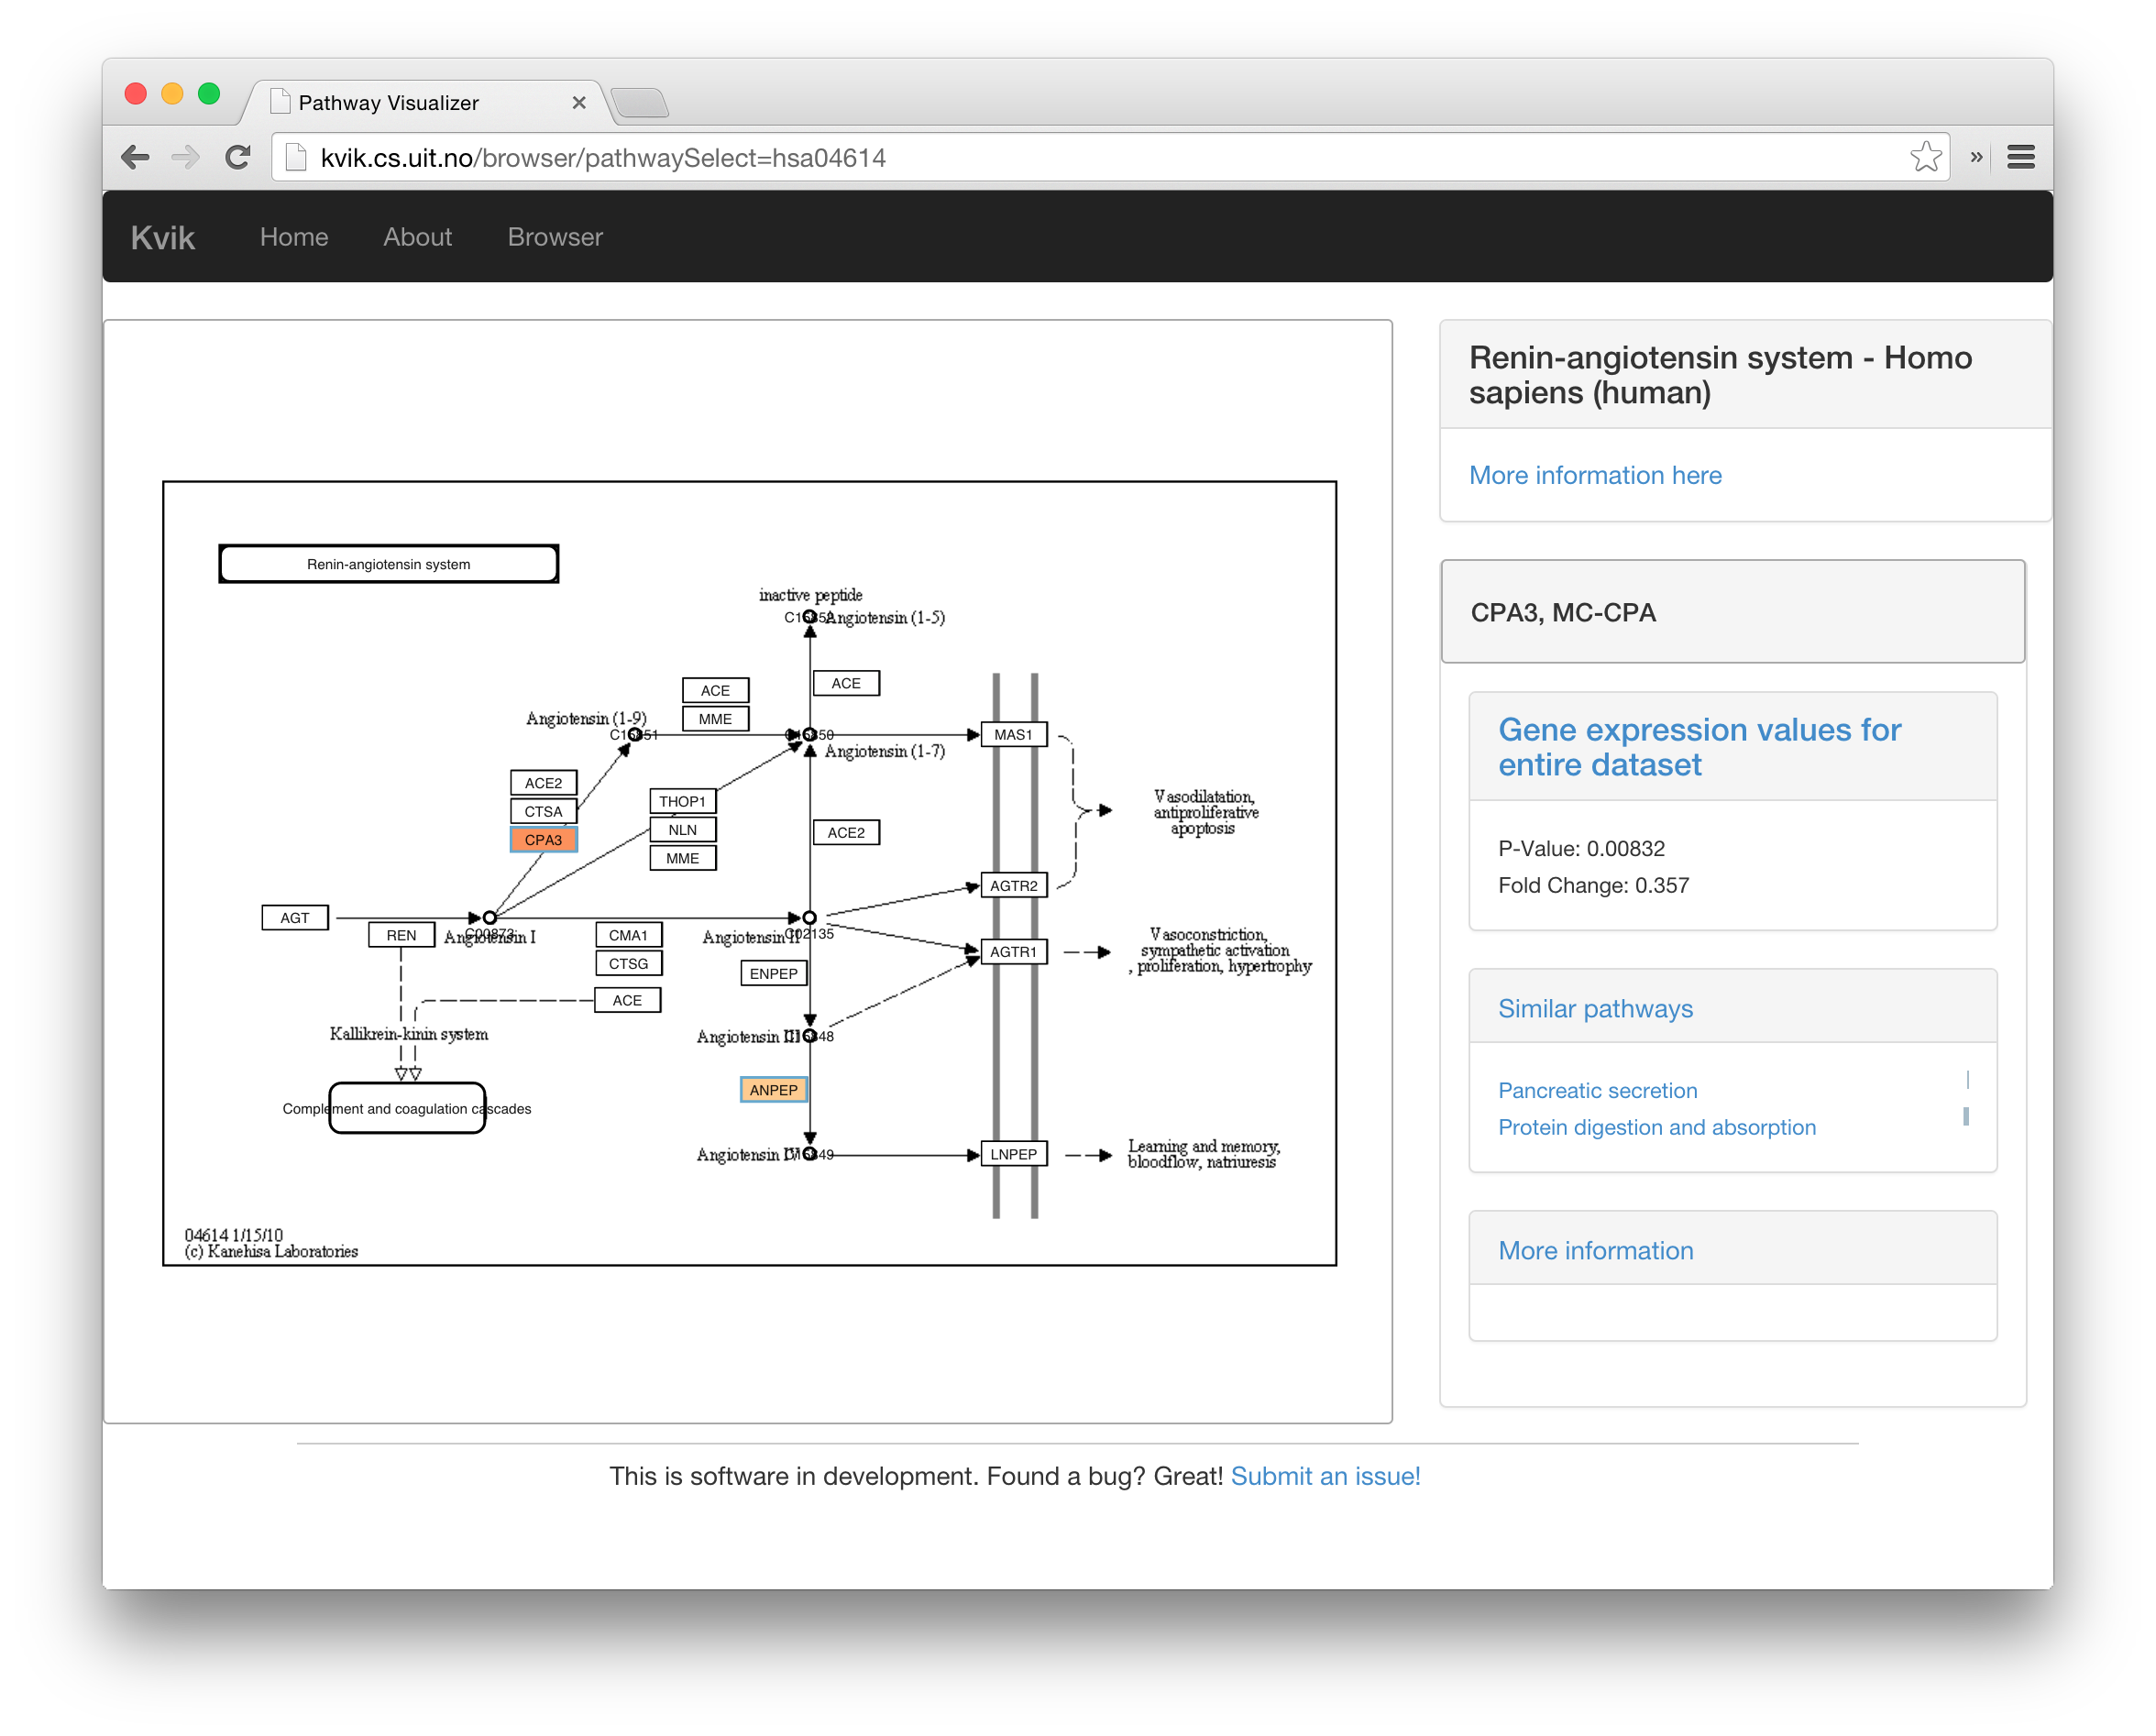
\includegraphics[width=\textwidth]{figures/kvikpwfig.png}
        \caption[Screenshot of the renin-angiotensin pathway in Kvik
        Pathways]{Screenshot of the renin-angiotensin pathway (KEGG pathway id
        hsa04614) in Kvik Pathways. Researchers can visually explore the
        pathways and read relevant information about genes in the right-hand
        panel.}
    \label{kvikpwfig}
    \end{centering} 
\end{figure}


\subsection{Architecture} 
Kvik Pathways has a three-tiered architecture of independent layers (Figure
\ref{fig:arch}). The browser layer consists of the web application for
exploring gene expression data and biological pathways. A front-end layer
provides static content such as HTML pages and stylesheets, as well as an
interface to the data sources with dynamic content such as gene expression
data or pathway maps to the web application. The backend layer contains
information about pathways and genes, as well as computational and storage
resources to process genomic data such as the \gls{nowac}  data repository. We
have used the packages in Kvik to develop the backend layer. These are discissed
in detail in Section \ref{kviksec}. 

The Data Engine in the backend layer provides an interface to the \gls{nowac}
data repository stored on a secure server on our local supercomputer. In Kvik
Pathways all gene expression data is stored on the computer that runs the Data
Engine. The Data Engine runs an R session accessible over remote procedure calls
(RPCs) from the front-end layer using RPy2\cite{rpy2} to interface with R. To
access data and run analyses the Data Interface exposes a HTTP \gls{api} to the
browser layer (Table \ref{interfacetable} provides the interfaces).

\begin{figure}[htb]
    \begin{centering}
    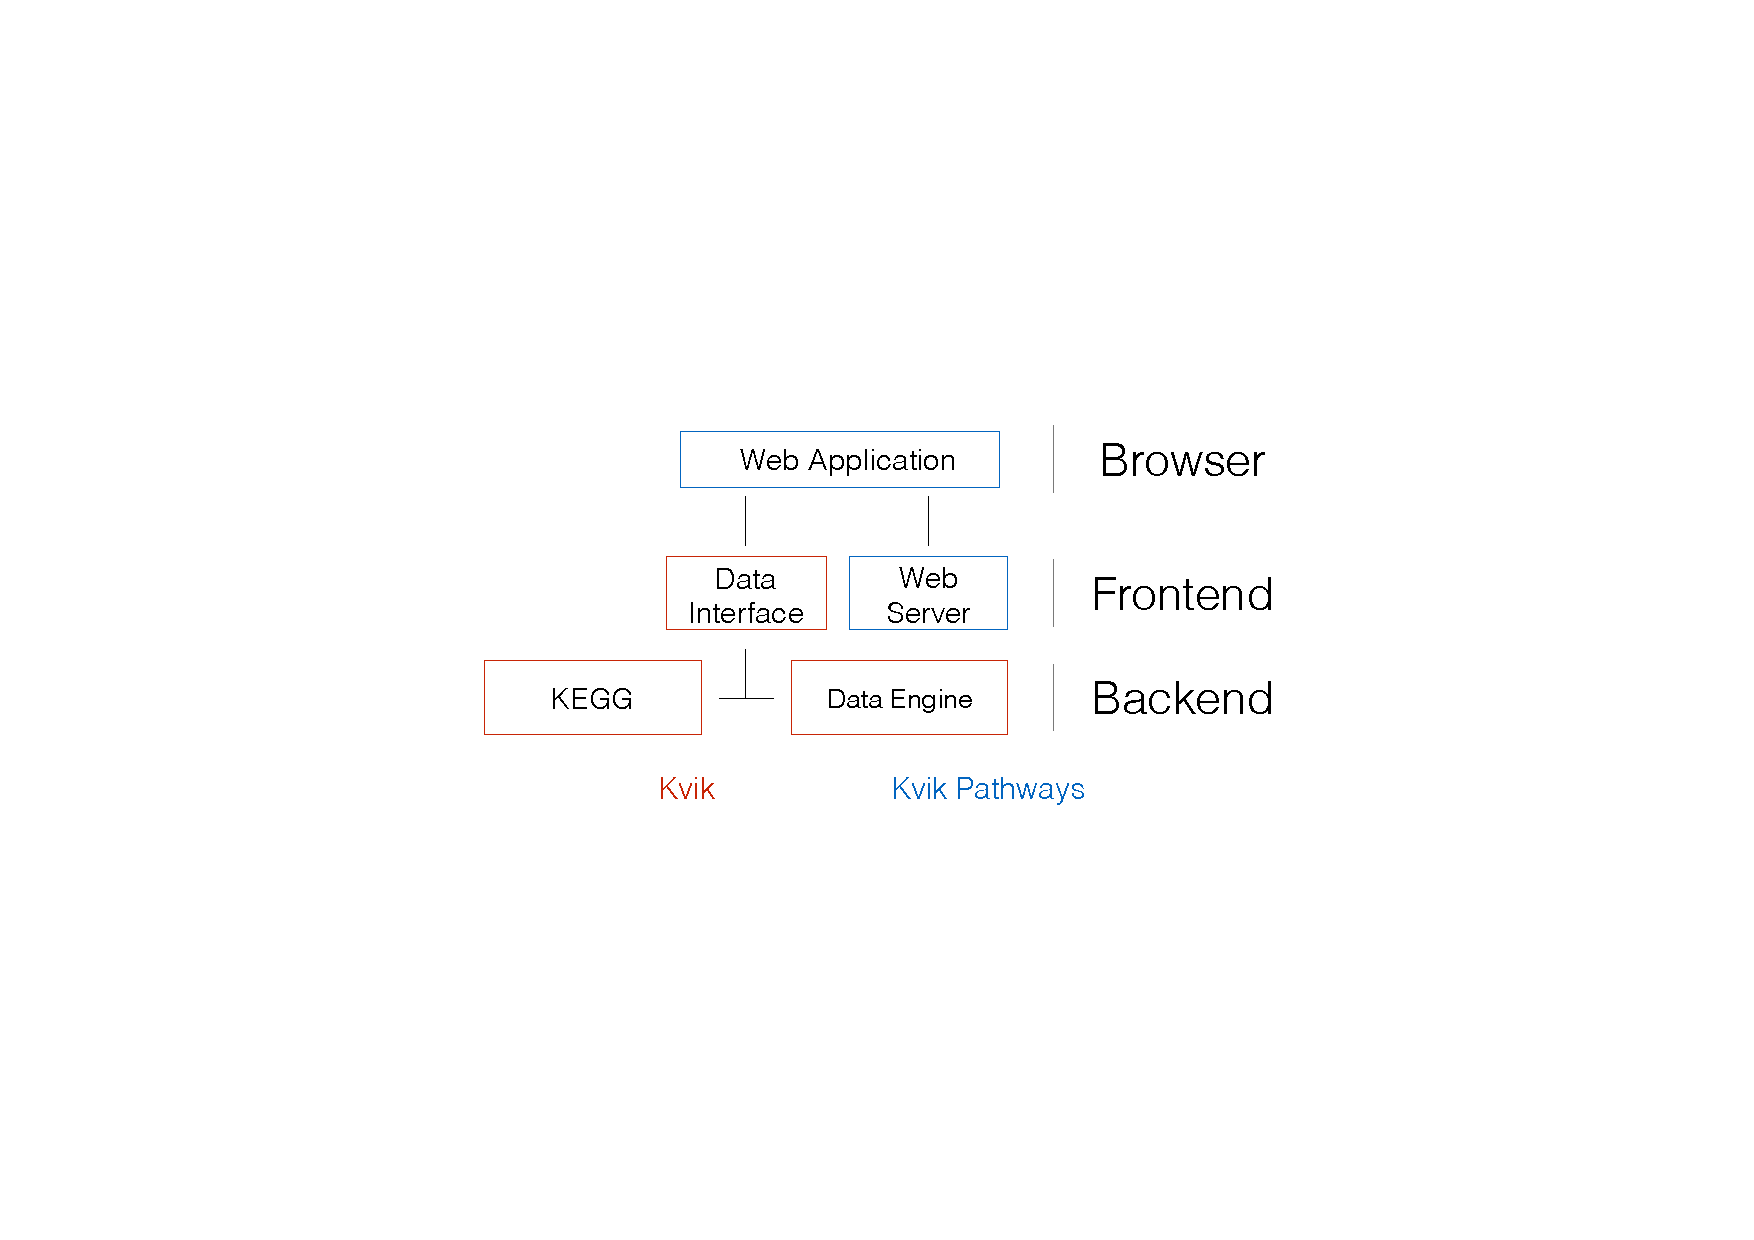
\includegraphics[width=\textwidth]{figures/archv2-name-fix.pdf}
    \caption{The three-tiered architecture of Kvik Pathways.} 
    \label{fig:arch}
    \end{centering} 
\end{figure}   

\begin{table}[!t]
\renewcommand{\arraystretch}{1.3}
\caption{
The REST interface to the Data Engine. For example, use \texttt{/genes/} to
    retrieve all available genes in our dataset.
}
\label{t1}
\centering\small
\begin{tabular*}{\linewidth}{@{\extracolsep{\fill}}p{0.025\linewidth}p{0.7\linewidth}@{}}
\hline
\bfseries URL & \bfseries Description\\
\hline
\emph{/fc/[genes...]} & Calculate and retrieve fold-change for the specified
    genes \\
\emph{/pvalues/[genes...]} & Calculate and retrieve $p$-values for the specified
    genes\\
\emph{/exprs/[genes...]} & Get the raw gene expression values from the dataset
    \\
\emph{/genes} & Get a list of all genes in the dataset \\
\hline
\end{tabular*}
    \label{interfacetable}
\end{table}

\subsection{Implementation} 
To create pathway visualizations the Kvik backend retrieves and parses the KEGG
Markup Language (KGML) representation and pathway image from KEGG databases
through its REST \gls{api}.\cite{kgml} This KGML representation of a pathway is an XML
file that contains a list of nodes (genes, proteins or compounds) and edges
(reactions or relations). Kvik parses this file and generates a JSON
representation that Kvik Pathway uses to create pathway visualizations.  Kvik
Pathways uses Cytoscape.js\cite{cytoscapejs} to create a pathway visualization
from the list of nodes and edges and overlay the nodes on the pathway image. See
Figure \ref{fig:how2pathway} for a graphical illustration of the process. To
reduce latency when using the \gls{kegg} \gls{rest} \gls{api}, we cache every
response on our servers.  We use the average fold change between the groups
(women with high or low plasma ratios of essential fatty acids) in the dataset
to color the genes within the pathway maps.  To highlight $p$-values, the
pathway visualization shows an additional colored frame around genes. We
visualize fold change values for individual samples as a bar chart in a side
panel.  This bar chart gives researchers a global view of the fold change in the
entire dataset. 

\begin{figure}[htb]
    \begin{centering}
    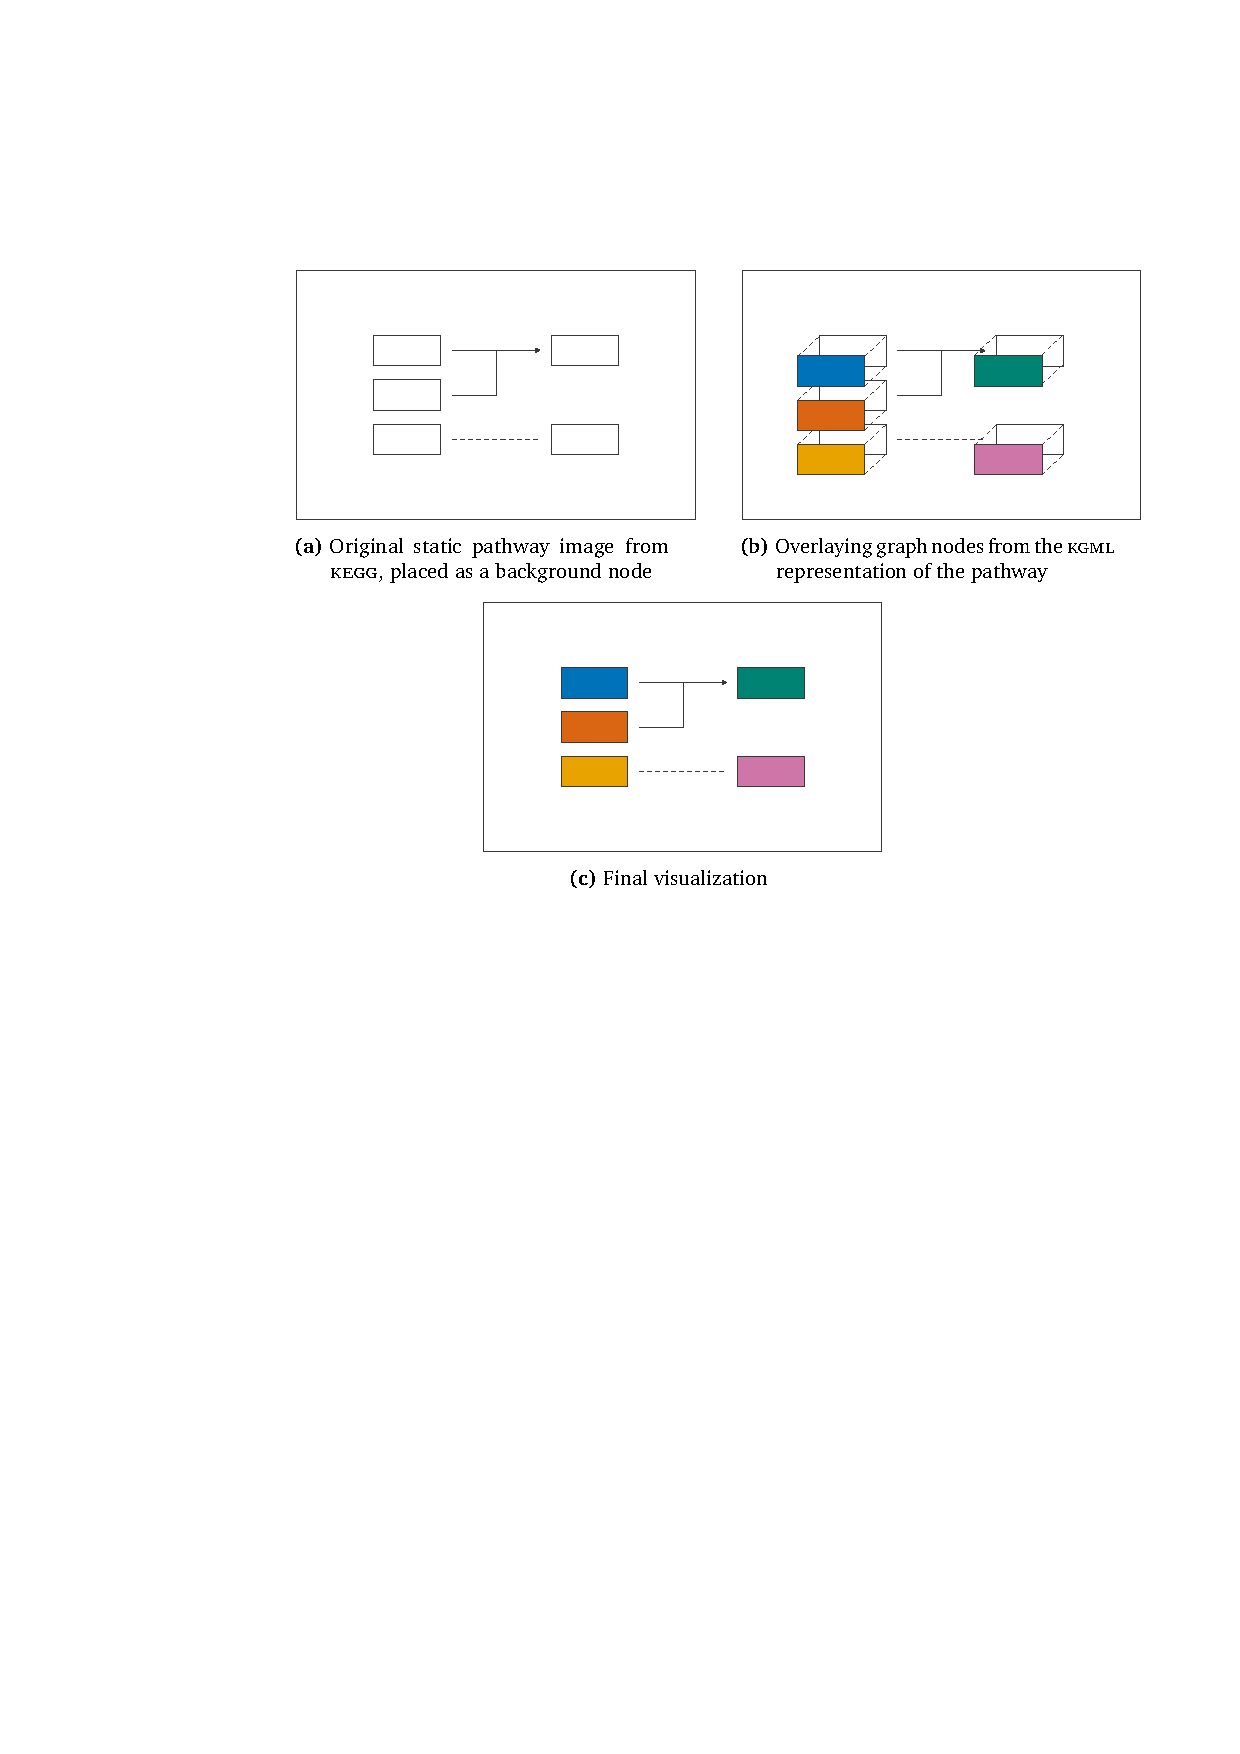
\includegraphics[width=\textwidth]{figures/how2pathway.pdf}
        \caption{Visualizing gene expression data on \gls{kegg} pathway maps.} 
    \label{fig:how2pathway}
    \end{centering} 
\end{figure}   

Kvik provides a flexible statistics backend where researchers can specify the
analyses they want to run to generate data for later visualization. For example,
in Kvik Pathways we retrieve fold change for single genes every time a pathway
is viewed in the application.  These analyses are run ad hoc on the backend
servers and generates output that is displayed in the pathways in the client's
web browser. The data analyses are implemented in an R script and can make use
of all available libraries in R, such as Bioconductor. 

Researchers modify this R script to, for example, select a normalization method,
or to tune the false discovery rate (FDR) used to adjust the $p$-values that
Kvik Pathways uses to highlight significantly differentially expressed genes.
Since Kvik Pathways is implemented as a web application and the analyses are run
ad hoc, when the analyses change, researchers get an updated application by
simply refreshing the Kvik Pathways webpage.

\subsection{Use Case: Analysis of Renin-Antiotensin Pathway}
As an example of practical use of Kvik Pathways, we chose one of the
significant pathways from the overlap analysis, the renin-angiotensin
pathway (Supplementary table S5 in \cite{olsen2013plasma}). The pathway
contains 17 genes, and in the pathway map we could instantly identify the
two genes that drive this result. The color of the gene nodes in the pathway
map indicates the fold change, and the statistical significance level is
indicated by the color of the node's frame.  We use this image of a
biological process to see how these two genes (and their expression levels)
are related to other genes in that pathway, giving a biologically more
meaningful context as compared to merely seeing the two genes on a list.

\section{Building Data Exploration Applications}\label{challengeref} 
Through the experiences developing the Kvik Pathways we identified a set of
components and features that are central to building data exploration
applications: 

\begin{enumerate}
    \item A low-latency language-independent approach for integrating, or
        embedding, statistical software, such as R, directly in a data
        exploration application. 
    \item A low-latency language-independent interface to online reference
        databases in biology that users can query to explore results in context
        of results in context of known biology. 
    \item A simple method for deploying and sharing the components of an
        application between projects. 
\end{enumerate} 


In the following sections we describe how we designed and implemented these in
Kvik, and how they later formed the bases of the \gls{sme} approach
that the \gls{mixt} web application builds upon. 

\section{Kvik}\label{kviksec}
Kvik is a collection of software packages in the Go programming language. It is
designed for developers that want to develop interactive data exploration
applications. It is the foundation in our two data exploration applications, and
has been iteratively developed through the last years. We have previously
refered to Kvik as Kvik Framework\cite{fjukstad2015kvik}, but we now refer to it
only as Kvik.  Kvik provides an interface to the R statistical programming
language, both as a stand-alone service, a client library, and through an
OpenCPU server. It provides an R-based pipelining tool that allows useres to
specify and run statistical analysis pipelines in R.  Kvik also contains a
Javascript package for visualizing KEGG pathways using d3.\cite{d3}  In addition
it provides an interface with online databases such as MsigDB\cite{msigdb} and
\gls{kegg}\cite{kegg}.

We used the experience building Kvik Pathways to completely re-design and
re-implement the R interface in Kvik. From having an R server that can run a
set of functions from an R script, it now has a clean interface to call any
function from any R package, not just retrieving data as a text string but in a
wide range of formats. We also re-built the database interface, which is now a
separate service. This makes it possible to leverage its caching capabilities
to improve latency. This transformed the application from being a single
monolithic application into a system that consists of a web application for
visualizing biological pathways, a database service to retrieve pathway images
and other metadata, and a compute service for interfacing with the gene
expression data in the \gls{nowac} cohort. We could then re-use the database and the
compute service in the MIxT application. 

We have used these packages to develop the \gls{sme} approach through services
that provide open interfaces to the R programming language and the online
databases.  We outline these services in \ref{micrservices}.  In short the
interfaces are accessible through an HTTP interface and can be used from any
platform.

\subsection{Microservices}\label{micrservices} 
We generalized our efforts from Kvik Pathways into the following design
principles for building applications in bioinformatics: 

\textbf{Principle 1}: Build applications as collections of language-agnostic
microservices. This enables re-use of components and does not enforce any
specific programming language on the user interfaces or the underlying
components of the application. 

\textbf{Principle 2}: Use software containers to package each service. This has
a number of benefits: it simplifies deployment, ensures that dependencies and
libraries are installed, and  simplifies sharing of services between
developers. 

\subsubsection{Compute Service}
We have built a compute service that provides an open interface directly to the
R programming language, thus providing access to a wealth of algorithm and
statistical analysis packages that exists within the R ecosystem.  
Application developers can use the compute service to execute specialized
analyses and retrieve results either as plain text or binary data such as plots.
By interfacing directly with R, developers can modify input parameters to
statistical methods directly from the user-facing application. 

The compute service offers three main operations to interface with R: i) to call
a function with one or more input parameters from an R package, ii) to get the
results from a previous function call, and iii) a catch-all term that both calls
a function and returns the results.  We use the same terminology as
OpenCPU\cite{opencpu} and have named the three operations Call, Get, and RPC
respectively. These three operations provide the necessary interface for
applications to include statistical analyses in the applications.

The compute service is implemented as an HTTP server that communicates with a
pre-set number of R processes to execute statistical analyses. 
At initiation of the compute service, a user-defined number of R worker sessions
are launched for executing analyses (default is 5).  
The compute service uses a round-robin scheduling scheme to distribute incoming
requests to the workers. We provide a simple FIFO queue for queuing of requests.
The compute service also provides the opportunity for applications to cache
analysis results to speed up subsequent calls. 

\subsubsection{Database Service} 
We have built a database service to interface with online biological databases.
The service provides a low latency interface, it minimizes the number of queries
to remote databases, and stores additional metadata to capture query parameters
and database information.  The database service provides an open HTTP interface
to biology databases for retrieving meta-data on genes and processes.  We
currently have packages for interfacing with E-utilities\cite{sayers2009entrez},
MSigDB, HGNC\cite{gray2014genenames}, and KEGG.

Both the compute and the databases service in Kvik build on the standard
\emph{net/http} package in the Go programming
language.\footnote{\url{golang.org}} The database service use
the \emph{gocache}\footnote{\url{github.com/fjukstad/gocache.}} package to cache
any query to an online database. In addition we deploy each service as Docker
containers.\footnote{Available at \url{hub.docker.com/r/fjukstad/kvik-r} and
\url{hub.docker.com/r/fjukstad/db}.}

\section{\gls{mixt}}
The \gls{mixt} system is an online web application for exploring and comparing
transcriptional profiles from blood and tumor samples. It provides users with an
interface to explore high-throughput gene expression profiles of breast cancer
tumor data with matched profiles from the patients blood. We have used the
microservices in Kvik to interface with statistical analyses and information
from online biology databases. 

\subsection{Analysis Tasks} 
To efficiently develop
the application we defined six analysis tasks (A1-A6) that the application
supports: 

\textbf{A1:} Explore co-expression gene sets in tumor and blood tissue.  Users
can explore gene expression patterns together with clinicopathological variables
(e.g. patient or tumor grade, stage, age) for each module.  In addition we
enable users to study the underlying biological functions of each module by
including gene set analyses between the module genes and known gene sets. 

\textbf{A2:} Explore co-expression relationships between genes. Users can
explore the co-expression relationship as a graph visualization. 
Here genes are represented in the network with nodes and edges represent 
statistically significant correlation in expression between the two end-points. 

\textbf{A3:} Explore relationships between modules from each tissue. We provide
two different metrics to compare modules, and the web application enables users
to interactively browse these relationships.  In addition to providing
visualizations the compare modules from each tissue, users can explore the
relationships, but for different breast cancer patient groups. 

\textbf{A4:} Explore relationships between clinical variables and modules. In
addition to comparing the association between modules from both tissues, users
also have the possibility to explore the association with a module and a
specific clinical variable. It is also possible to explore the associations
after first stratifying the tumors by breast cancer subtype (an operation that
is common in cancer related studies to deal with molecular heterogeneity).

\textbf{A5:} Explore association between user-submitted gene lists and computed
modules. We want to enable users to explore their own gene lists to explore
them in context of the co-expression gene sets. The web application must handle
uploads of gene lists and compute association between the gene list and the MIxT
modules on demand. 

\textbf{A6:} Search for genes or gene lists of interest. To facilitate faster
lookup of genes and biological processes, the web application provides a search
functionality that lets users locate genes or gene lists and show association to
the co-expression gene sets. 

\subsection{Architecture} 
We structured the MIxT application with a separate view for each analysis task.
To explore the co-expression gene sets (\textbf{A1}), we built a view that
combines both static visualizations from R together with interactive tables for
gene overlap analyses. Figure \ref{fig_first_case} shows the web page presented
to users when they access the co-expression gene set 'darkturquoise' from blood.
To explore the co-expression relationship between genes (\textbf{A2}) we use an
interactive graph visualization build with Sigma.\cite{sigmajs}
We have built visualization for both tissues, with graph sizes of 2705 nodes and
90 348 edges for the blood network, and 2066 nodes and 50 563 edges for the
biopsy network. 
To visualize relationships between modules from different tissues (\textbf{A3}),
or their relationship to clinical variables (\textbf{A4}) we built a heatmap
visualization.
We built a simple upload page where users can specify their gene sets
(\textbf{A5}). The file is uploaded to the web application which redirects it to
a backend service that runs the analyses. Similarly we can take user input to
search for genes and processes (\textbf{A6}).

\begin{figure}[h!]
\centering
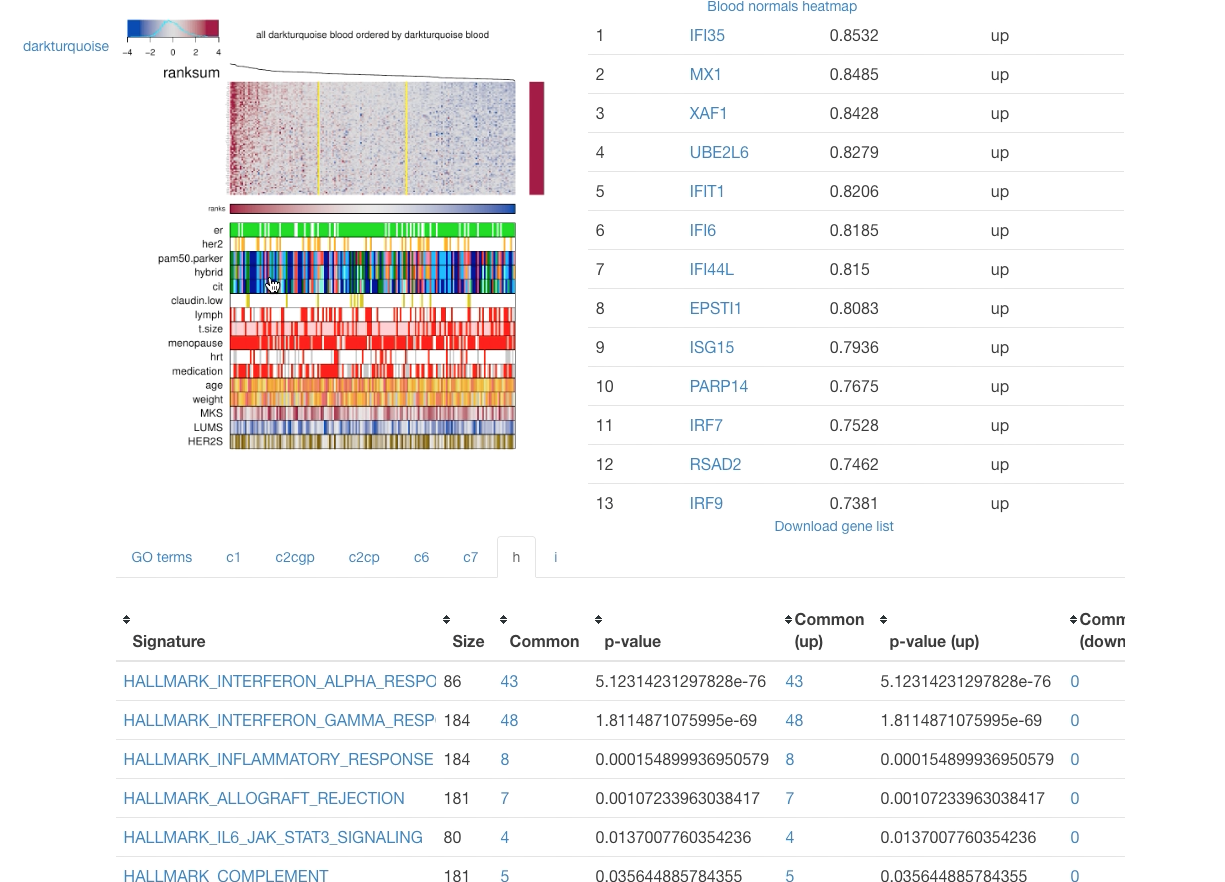
\includegraphics[width=\columnwidth]{figures/module.png}
    \caption[MIxT module overview page.]{MIxT module overview page.
The top left panel
contains the gene expression heatmap for the module genes. The top right panel
contains a table of the genes found in the module. The bottom panel contains the
results of gene overlap analyses from the module genes and known gene sets from
MSigDB.}
\label{fig_first_case}
\end{figure} 

For the original analyses we built an R package, mixtR,\footnote{Available
online at \url{github.com/vdumeaux/mixtR.}} with the statistical methods and
static visualizations for identifying associations between modules across
tissues. The mixtR package is based on the \gls{wgcna} R package to compute the
correlation networks\cite{langfelder2008wgcna}.  To make the results more easily
accessible we built a web application
that interfaces with the R package, but also online databases to retrieve
relevant metadata. To make it possible to easily update or re-implement parts of
the system without effecting the entire application, and we developed it using a
microservice architecture. The software containers allowed the application to be
deployed on a wide range of hardware, from local installations to cloud systems.

\subsection{Implementation} 
From the six analysis tasks we designed and implemented MIxT as a web
application that integrates statistical analyses and information from biological
databases together with interactive visualizations. Figure \ref{kvik-mixt} shows
the system architecture of MIxT which consists of three parts i) the
web application itself containing the user-interface and visualizations; ii) the
compute service performing the MIxT analyses developed in an R package,
delivering data to the web application; and iii) the database service providing
up-to-date information from biological databases.  Each of these components run
in Docker containers making the process of deploying the application simple. 

\begin{figure}[h!]
\centering
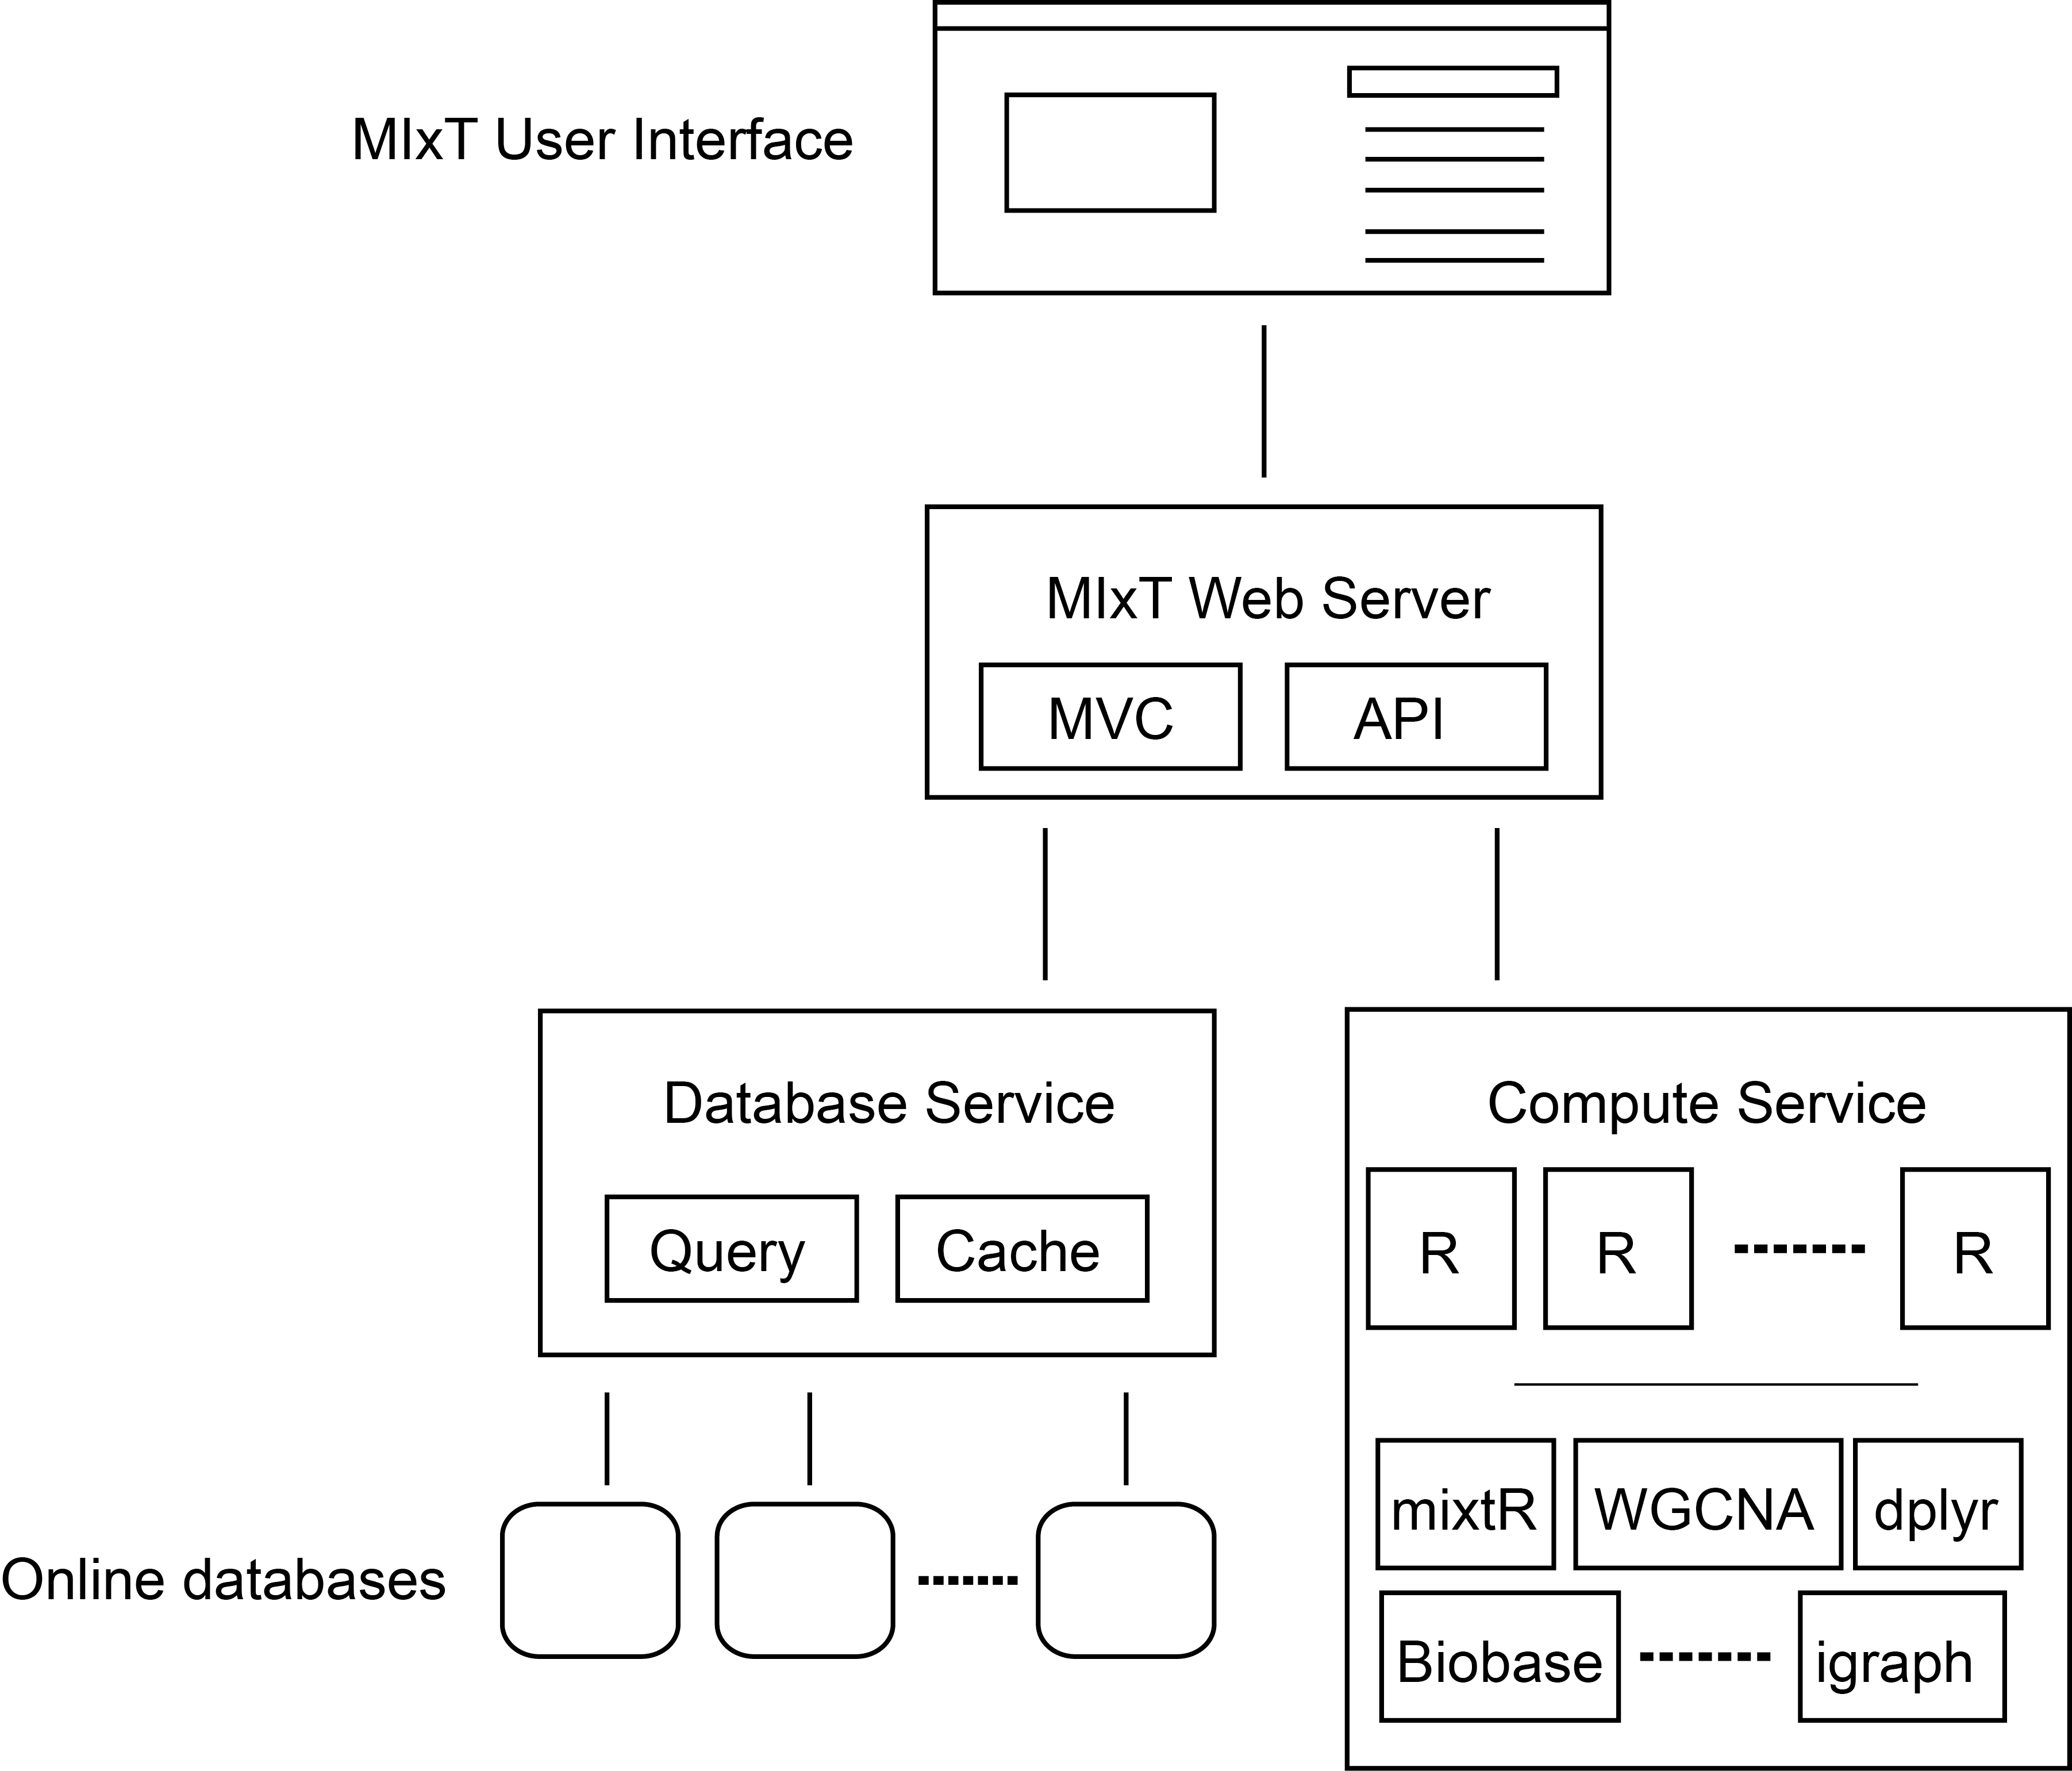
\includegraphics[scale=0.4]{figures/mixt-architecture.png}
    \caption[The architecture of the MIxT system.]{The architecture of the MIxT
    system. It consists of a web application, the hosting web server, a database
    service for retrieving metadata and a compute service for performing
    statistical analysis. Note that only the web application and the R package
    are specific to MIxT, the rest of the components can be reused in other
    applications.} 
\label{kvik-mixt}
\end{figure} 

The web application is hosted by a custom web server. This web server is
responsible for dynamically generating the different views based on data from
the statistical analyses and biological databases, and serve these to users. It
also serves the different JavaScript visualization libraries and style sheets. 

\subsection{Evaluation} 
We evaluate the MIxT application by investigating response times for a set of
queries to each of its two supporting services. 

To evaluate the database service we measure the query time for retrieving
information about a specific gene with and without caching.\footnote{More
details online at \url{github.com/fjukstad/kvik}.} This
illustrates how we can improve performance in an application by using a database
service rather than accessing the database directly. 
We use a AWS EC2 \emph{t2.micro}\footnote{See
\url{aws.amazon.com/ec2/instance-types} for more information about AWS EC2
instance types.} instance to host and evaluate the database service.  The
results in Table \ref{db} confirm a significant improvement in response time
when the database service caches the results from the database lookups. In
addition by serving the results out of cache we reduce the number of queries to
the online database down to one. 

\begin{table}[h]
\centering
    \caption{Time to retrieve a gene summary for a single gene, comparing
    different number of concurrent requests.}
    \begin{tabular}{| l | c | c | c | c | c | }
        \hline 
        & 1 & 2 & 5 & 10 & 15 \\ 
      \hline			
      No cache & 956ms & 1123ms & 1499ms & 2147ms & 2958ms\\
      \hline
      Cache & 64ms & 64ms & 130ms & 137ms & 154ms\\
      \hline  
    \end{tabular}
\label{db}
\end{table} 

We evaluate the compute service by running a benchmark consisting of two
operations: first generate a set of 100 random numbers, then plot them and
return the resulting visualization.\footnote{More details at
\url{github.com/fjukstad/kvik}.} We use two \emph{c4.large} instances on AWS EC2
running the Kvik compute service and OpenCPU base docker containers. The servers
have caching disabled.  Table \ref{kvikopencpucomparison} shows the time to
complete the benchmark for different number of concurrent connections. We see
that the compute service in Kvik performs better than the OpenCPU\footnote{Built
using the \textit{opencpu-server} Docker image.} alternative. We believe that
speedup is because we keep a pool of R processes that handle requests. In
OpenCPU a new R process is forked upon every request that results in any
computation executed in R. Other requests such as retrieving previous results do
not fork new R processes. 

In summary our results show that the interface to the R programming language
provides faster latencies, and that implementing a service for database lookups
have clear benefits with regards to latency. 

\begin{table}[h]
\centering
    \caption{Time to complete the benchmark with different number of
    concurrent connections.}
    \begin{tabular}{| l | c | c | c | c | c | }
        \hline 
       & 1 & 2 & 5 & 10 & 15 \\ 
      \hline			
      Kvik & 274ms & 278ms & 352ms & 374ms & 390ms\\
      \hline
      OpenCPU & 500ms & 635ms & 984ms & 1876ms & 2700ms\\
      \hline  
    \end{tabular}
\label{kvikopencpucomparison}
\end{table} 

\subsection{Tumor Epithelium-Stroma Interactions in Breast Cancer}
In addition to the MIxT web application for exploring the link between breast
tumor and primary blood, we have also deployed a web application that
investigates the link in another dataset\cite{boersma2008stromal} We have
deployed the application online at \url{mixt-tumor-stroma.bci.mcgill.ca}. The
web application is identical, but the underlying dataset is different.

\subsection{air:bit}
We have also used the microservice architecture in an application where users
can upload and explore air pollution data from Northern
Norway.\cite{fjukstad2018low} In the project, air:bit, students from upper
secondary schools in Norway collect air quality data from sensor kits that they
have built and programmed. The web application lets the students upload data
from their kits, and provides a graphical interface for them to explore data
from their own, and other participating schools. The system consists of a web
server frontend that retrieves air pollution data from a backend storage system
to build interactive visualizations. It also integrates the data with other
sources such as the Norwegian Institute for Air Research and the The Norwegian
Meteorological Institute. 

    
\section{Related Work}\label{sec:int:rel}
There are different technologies for developing different data exploration
applications. We have surveyed comparable applications for exploring similar
datasets to the ones we describe in this chapter, and underlying technology for
developing these applications. 

\subsection{Applications} 
There are a wealth of resources for exploring biological pathway maps.
KEGG\cite{kegg} provides a large collection of static pathway maps that users
can navigate through and download. They provide both static images of the
pathways, as well as a textual representation of the pathway in the \gls{kgml}.
\gls{kegg} provides a \gls{rest} \gls{api} that
developers can use to integrate both pathway maps and other information in their
application. In \gls{kegg} Pathways we heavily rely on the data from \gls{kegg}. 
Reactome is an open-source peer-reviewed online knowledgebase of biomolecular
pathways.\cite{fabregat2018reactome} Users can download the entire graph
database or explore it in their pathway visualization tool. They have not yet
made an \gls{api} open for developers, but are planning to do so. Libraries such as
KEGGViewer\cite{villaveces2014keggviewer} allow developers to integrate pathway
visualization maps in web applications, but these are generated using the
\gls{kgml} representations, that do not include additional visual cues found in
the static \gls{kegg} pathway maps.  enRoute\cite{partl2012enroute} is a desktop
application for exploring pathway maps from \gls{kegg} that combines the static
pathway maps from \gls{kegg} in an interactive application. Pathview is both an
R package and an online web application for exploring pathway
maps.\cite{luo2017pathview} The online web application is built on top of the R
package and provides the same functionality, but through a \gls{gui}. Pathway
generates static pathway visualizations based on pathway maps from \gls{kegg}. 

There are few related systems that provide visualizations of \gls{wgcna}
results. The R package from the original paper provides a wide range of
different utility functions for visualization, but it is only accessible within
the R environment.  The \gls{wgcna} Shiny app\footnote{Online a
shiny.etriks.org/wgcna} is an interactive application for performing, and
exploring results from, \gls{wgcna}.  The online version allows users to explore
two demo datasets, and it is possible to download the application and change out
the datasets locally. In short it is a web implementation of the \gls{wgcna} R
package that allows users without any R experience perform \gls{wgcna}. It is
developed and maintained by the eTRIKS platform.\cite{bussery2018etriks}

\subsection{Technology} 
OpenCPU is a system for embedded scientific computing and reproducible
research.\cite{opencpu} Similar to the compute service in Kvik, it offers an
HTTP \gls{api} to the R programming language to provide an interface with
statistical methods. It allows users to make function calls to any R package and
retrieve the results in a wide variety of formats such as JSON or PDF. OpenCPU
provides a JavaScript library for interfacing with R, as well as Docker
containers for easy installation, and has been used to build multiple
applications.\footnote{\url{opencpu.org/apps.html}.}. The compute service in
Kvik follows many of the design patterns in OpenCPU. Both systems interface with
R packages using a hybrid state pattern over HTTP. Both systems provide the same
interface to execute analyses and retrieve results.  Because of the similarities
in the interface to R in Kvik we provide packages for interfacing with our own R
server or OpenCPU R servers.

Shiny is a web application framework for R\footnote{\url{shiny.rstudio.com}.}
It allows developers to build web applications in R without having to have any
knowledge about HTML, CSS, or Javascript. While it provides an easy alternative
to build web applications on top of R, it cannot be used as a service in an
application that implements the user-interface outside of R.  

Renjin is a JVM-based interpreter for the R programming language.\cite{renjin}
It allows developers to write applications in Java that interact directly with R
code. This makes it possible to use Renjin to build a service for running
statistical analyses on top of R. One serious drawback is that existing R
packages must be re-built specifically for use in Renjin. 

Cytoscape is an open source software platform for visualizing complex networks
and integrating these with any type of attribute
data.\cite{shannon2003cytoscape} Through a Cytoscape App, cyREST, it allows
external network creation and analysis through a REST \gls{api}\cite{ono2015cyrest},
making it possible to use Cytoscape as a service.  To bring the visualization
and analysis capabilities to the web applications the creators of Cytoscape have
developed Cytoscape.js\footnote{\url{js.cytoscapejs.org}.}, a JavaScript library
to create interactive graph visualizations.  Another alternative for biological
data visualization in the web browser is BioJS It provides a community-driven
online repository with a wide range components for visualizing biological data
contributed by the bioinformatics community.\cite{gomez2013biojs} BioJS builds
on node.js\footnote{\url{nodejs.org}.} providing both server-side and
client-side libraries. In MIxT we have opted to build the visualizations from
scratch using sigma.js and d3 to have full control over the appearance and
functionality of the visualizations. 

\section{Discussion}
In this chapter we have given a description of how we successfully built two
data exploration applications for high-throughput biological datasets. We have
iteratively developed these and ended up with an approach that allows us to
develop applications from disparate systems. 

As we have seen in \ref{sec:int:rel} there are many applications that provide
visualization tools to view and browse pathway maps, most of which
use \gls{kegg} as its main data source. The applications then either reuse
the pathway maps, and augment them with gene expression data, or use the
underlying \gls{kgml} description and generate their own graphical
representation with gene expression data. Using the first method will provide
the additional visual ques found in the static pathway images, but the
visualizations are less flexible with regards to node and edge placement. Using
the second method provides more flexible graphs with regards to layout, but this
could make the visualizations less familiar to the users interpreting them. We
believe that using the techniques that provides the most familiar representation
of the pathways are easiest to interpret for the users. 

With both of these techniques the underlying gene expression datasets are loaded
using different techniques. Most systems allow users to specify gene expression
values in some table format and render the values in top of the pathway map.
These values are typically the end result of a long analysis process which users
have to track manually. By integrating the visualization with the analysis
software, typically R, it is possible to access data from anywhere in the
analysis process, and also provide detailed information to the user regarding
the underlying data analysis process.  What separates our approach in Kvik
Pathways to the other related systems, is this integration between the end
visualization and the gene expression datasets. By using Kvik it is possible to
develop applications that automatically lets users access the underlying data
analysis, and thereby connecting the interpretable end results with the
analyses. 

The \gls{wgcna} Shiny app provides similar visualizations as our MIxT web
application, but the application is limited to that of a web application. Shiny
lets its users develop applications written purely in R, including the backend
server and the user interfaces. In MIxT we developed an R package with a set of
resources, or endpoints, for application developers to access through a Kvik R
service. This allows application developers to develop the user-facing logic
using any type of technology or framework. The resources are available through
the HTTP API in Kvik making it possible for anyone to develop an
application on top of the dataset and analyses. We acknowledge the strength of R
for data analysis, but not for developing complex user-facing applications. 

There are different arguments for reusing and sharing microservices over
libraries in bioinformatics applications, that would justify the cost of hosting
an maintaining a set of distributed microservices.  We argue that applications
that require large computational or storage resources can benefit from the
microservices approach because the applications can share the underlying compute
infrastructure between multiple applications and users.  This makes it possible
to deploy an application on a lightweight system that uses a common service for
computation and storage. In addition, benefits such as using different
programming languages for a single application, and packaging a microservice as
a software container, help to outweigh the operational burden related to using
microservices to build applications. 

Of the related systems, OpenCPU provides the most similar interface to analyze
datasets as the R interface in Kvik. While we started to explore OpenCPU for use
in our applications, we found through our benchmarking that it did not provide
satisfactory performance for our applications. It does however provide a richer
set of functionality, such as exporting data in many more formats and running
user-submitted scripts. We did not find it necessary for these additions and
implemented our own R interface that could provide the necessary interface for
us to implement data exploration applications. 

We have reused the microservices for running statistical analyses and
fetch biological metadata, and share these between applications. This makes it
possible for multiple applications to use one or more powerful servers for
hosting the services. In the case of statistical analyses we simply install the
necessary R packages for each application on the compute service and run it as
we would for one single application. 

\section{Future Work} 
We hope to continue development on applications for interactively exploring
biological datasets. Through our approach, and especially the interface to R, 
we are now able to develop applications that can use any function or retrieve
datasets from any R package. This includes the \texttt{nowac} package in
Chapter \ref{biodata}. We believe that there is a large potential in the
available datasets, and that researchers would benefit from being able to
interactively explore these. 

\subsection{MIxT} 
We intend to address few points in future work, both in the
MIxT web application as well as the supporting microservices.  The first issue
is to improve the user experience in the MIxT web application.  Since it is
executing many of the analyses on demand, the user interface may seem
unresponsive. We are working on mechanisms that gives the user feedback when the
computations are taking a long time, but also reducing analysis time by
improving the performance the underlying R package. The database service
provides a sufficient interface for the MIxT web application. While we have
developed the software packages for interfacing with more databases, these
haven't been included in the database service yet. In future versions we aim to
make the database service an interface for all our applications.  We also aim to
improve how we capture data provenance. We aim to provide database versions and
meta-data about when a specific item was retrieved from the database. 

One large concern that we haven't addressed in this chapter is security. In
particular one security concern that we aim to address in Kvik is the
restrictions on the execution of code in the compute service. We aim to address
this in the next version of the compute service, using methods such as
AppArmor\cite{apparmor} that can restrict a program's resource access. In
addition to code security we will address data access, specifically put
constraints on who can access data from the compute service.  We also aim to
explore different alternatives for scaling up the compute service.  Since we
already interface with R we can use the Sparklyr\cite{sparklyr} or
SparkR\cite{sparkr} packages to run analyses on top of
Spark.\cite{zaharia2012resilient} Using Spark as an execution engine for data
analyses will enable applications to explore even larger datasets.

\section{Conclusion}
We have designed an approach for building data exploration applications in
cancer research. We first implemented Kvik Pathways, a web application for
exploring a gene expression dataset in the context of pathway maps. We used our
experiences to generalize our efforts into a set of central components that
these types of applications require. Further we realized these in our \gls{sme}
approach implemented as a set of microservices.  Using these services we have
built a web application, MIxT, that integrates statistical analyses, interactive
visualizations, and data from biological databases. While we have used our
approach to build an application in cancer research, we believe that the
microservice architecture can be used to build data exploration systems in other
disciplines as well. 

In summary, our primary lesson learned from the experiences with develop our two
applications, is to compose and develop a data exploration system from
independent parts.  We chose to implement our systems using three separate
services. A compute service to provide statistical analyses, a database service
to provide access to biological databases, and the user interface. This makes it
possible to quickly re-implement parts of the system, but also allow others to
interface with its underlying components, not just the user interface. 

\chapter{Deep Analysis Pipelines}\label{pipeline}  
In this chapter we discuss our approach to analyzing high-throughput genomic
datasets through deep analysis pipelines, and its implementation in 
walrus.\cite{walrus} We also evaluate the performance of walrus and show its
usefulness in a precision medicine setting. While walrus was developed in this
context we also show its usefulness in other areas, specifically for
\gls{rna}-seq analyses. 

\section{Use Case and Motivation} 
Precision medicine uses patient-specific molecular information to diagnose and
categorize disease to tailor treatment to improve health
outcome.\cite{national2011toward} Important goals in precision medicine are to
learn about the variability of the molecular characteristics of individual
tumors, their relationship to outcome, and to improve diagnosis and
therapy.\cite{tannock2016limits} Cancer institutions are therefore now
offering dedicated personalized medicine programs. 

For cancer, high throughput sequencing is an emerging technology to facilitate
personalized diagnosis and treatment since it enables collecting high quality
genomic data from patients at a low cost. Data collection is becoming cheaper,
but the downstream computational analysis is still time-consuming and thereby
a costly part of the experiment.  This is because of the manual efforts to set
up, analyze, and maintain the analysis pipelines. These pipelines consist of
many steps that transform raw data into interpretable
results.\cite{diao2015building} These pipelines often consists of in-house or
third party tools and scripts that each transform input files and produce some
output. Although different tools exist, it is necessary to carefully explore
different tools and parameters to choose the most efficient to apply for a
dedicated question.\cite{servant2014bioinformatics} The complexity of the tools
vary from toolkits such as the \gls{gatk} to small custom \texttt{bash} or
\texttt{R} scripts.  In addition, some tools interface with databases whose
versions and content will impact the overall result.\cite{sboner2015primer}

Improperly developed analysis pipelines for precision medicine may generate
inaccurate results, which may have negative consequences for patient
care.\cite{roy2017standards} Users and clinicians therefore need systems that
can track pipeline tool versions, their input parameters, and data. Both to
thoroughly document what produced the final clinical reports, and to iteratively
improve the quality of the pipeline during development. Because of the
iterative process of developing the analysis pipeline, it is necessary to use
analysis tools that facilitate modifying pipeline steps and adding new ones with
little developer effort.

Developing a system that enables researchers to write and share reproducible
analysis pipelines will enable the scientific community to analyze
high-throughput genomic datasets faster and more unified. By combining
versioning of datasets and pipeline configurations, a pipeline management system
will provide interpretable and reproducible results long after the initial data
analysis will have completed. These features will together promote reproducible
science and improve the overall quality of the analyses. 

\subsection{Initial Data Analysis Pipeline} 
We have analyzed DNA sequence data from a breast cancer patient's
primary tumor and adjacent normal cells to identify the molecular signature of
the patient's tumor and germline. When the patient  later relapsed we analyzed
sequence data from the patient's metastasis to provide an extensive comparison
against the primary and to identify the molecular drivers of the patient's
tumor. 

We used \gls{wgs} to sequence the primary tumor and adjacent normal cells at an
average depth of 20, and \gls{wes} at an average depth of 300. The biological
samples were sequenced at the Genome Quebec Innovation Centre, and we stored the
raw datasets on our in-house server.  From the analysis pipelines we generated
reports with end results, such as detected somatic mutations, that was
distributed to both the patient and the treating oncologists. These could be
used to guide diagnosis and treatment, and give more detailed insight into both
the primary and metastasis.  When the patient relapsed we analyzed \gls{wes}
data using our own pipeline manager, \texttt{walrus}, to investigate the
metastasis and compare it to the primary tumor. 

For the initial \gls{wgs} analysis we developed a pipeline to investigate
somatic and germline mutations based on Broad Institute's best practices. We
developed the analysis pipeline on our in-house compute server using a
\emph{bash} script under version control with \emph{git} to track changes as we
developed the analysis pipeline. The pipeline consisted of tools including
picard\cite{picard}, fastqc\cite{fastqc}, trimmomatic\cite{trimmomatic}, and the
\gls{gatk}.\cite{gatk} While the analysis tools themselves provide the necessary
functionality to give insights in the disease, 
% LAB: Kan vi gi ett illustrerende eksempel på hvorfor dette var viktig i
% "motivating use case". Ellers blir det rart hvis hovedpoenget med walrus ikke
% var motivert.
ensuring that the analyses could be fully reproduced later left areas in need of
improvement.

We chose a command-line script over more complex pipelining tools or workbenches
such as Galaxy\cite{goecks2010galaxy} because of its fast setup time on our
available compute infrastructure, and familiar interface. More complex systems
could be beneficial in larger research groups with more resources to compute
infrastructure maintenance, whereas command-line scripting languages require
little infrastructure maintenance over normal use. In addition, while there are
off-site solutions for executing scientific workflows, analyzing sensitive data
often put hard restrictions on where the data can be stored and analyzed.

After we completed the first round of analyses we summarized our efforts and
noted features that pipeline management systems should satisfy: 
\begin{itemize}
    \item  Datasets and databases should be under version control and stored
        along with the pipeline description. In the analysis script we
        referenced to datasets and databases by their physical location on a
        storage system, but these were later moved without updating the pipeline
        description causing extra work. A solution would be to add the data to
        the same version control repository hosting the pipeline description.
    \item The specific pipeline tools should also be kept available for
        later use. Often in bioinformatics, just installing a tool is a
        time-consuming process because of their many dependencies. 
    \item It should be easy to add new tools to an existing
        pipeline and execution environment. This includes installing the specific
        tool and adding to an existing pipeline. Bundling tools within software
        containers, such as Docker, and hosting them on an online registry
        simplifies the tool installation process since the only requirement is
        the container runtime.
    \item While bash scripts have their
        limitations, using a well-known format that closely resembles the normal
        command-line use clearly have its advantages. It is easy to understand
        what tools were used, their input parameters, and the data flow.
        However, from our experience when these analysis scripts grow too large
        they become too complex to modify and maintain. 
    \item While there are new and promising state-of-the art pipeline
        managers, many of these also require state-of-the-art computing
        infrastructure to run. This may not be the case at cancer research
        and clinical institutions. 
\end{itemize} 

The above problem areas are not just applicable to our research group, but
common to other research and precision medicine projects as well. Especially
when hospitals and research groups aim to apply personalized medicine efforts to
guide therapeutic strategies and diagnosis, the analyses will have to be able to
be easily reproducible later. We used the lessons learned to  design and
implement \texttt{walrus}, a command line tool for developing and running data
analysis pipelines. It automatically orchestrates the execution of different
tools, and tracks tool versions and parameters, as well as datasets through the
analysis pipeline. It provides users a simple interface to inspect differences
in pipeline runs, and retrieve previous analysis results and configurations. In
the remainder of the paper we describe the design and implementation of
\texttt{walrus}, its clinical use, its performance, and how it relates to other
pipeline managers. 

\section{\texttt{walrus}} 
\texttt{walrus} is a tool for developing and executing data analysis pipelines.
It stores information about tool versions, tool parameters, input data,
intermediate data, output data, as well as execution environments to simplify
the process of reproducing data analyses. Users write descriptions of their
analysis pipelines using a familiar syntax and \texttt{walrus}  uses this
description to orchestrate the execution of the pipeline. In \texttt{walrus}  we
package all tools in software containers to capture the details of the different
execution environments. While we have used \texttt{walrus} to analyze
high-throughput datasets in precision medicine, it is a general tool that can
analyze any type of data, e.g. image datasets for machine learning. It has few
dependencies and runs on any platform that supports Docker containers. While
other popular pipeline managers require the use of cluster computers or cloud
environment, we focus on single compute nodes often found in clinical
environments such as hospitals. 

\texttt{walrus} is implemented as a command-line tool in the Go programming
language. We use the popular software container implementation
Docker\cite{docker} to provide reproducible execution environments, and
interface with git together with \texttt{git-lfs}\cite{gitlfs} to version control
datasets and pipeline descriptions. By choosing Docker and git we have built a
tool that easily integrates with current bioinformatic tools and workflows. It
runs both natively or within its own Docker container to simplify its
installation process.

With \texttt{walrus} we target pipeline developers that use command-line tools
and scripting languages to build and run analysis pipelines. Users can use
existing Docker containers from sources such as
BioContainers\cite{biocontainers} or build containers with their own tools.  We
integrate with the current workflow using git to version control analysis
scripts, and use \texttt{git-lfs} for versioning of datasets as well. We have
designed the pipeline description format resembles the command line syntax as
much as possible. This is one of the major strengths of walrus. It uses a
familiar syntax and format, and does not require the users to explicitly
declare which files in the pipeline to version control. 


\subsection{Pipeline Configuration}
Users configure analysis pipelines by writing pipeline description files in a
human readable format such as \gls{json} or \gls{yaml}. A pipeline description
contains a list of stages, each with inputs and outputs, along with optional
information such as comments or configuration parameters such as caching rules
for intermediate results. Listing \ref{examplelisting} shows an example pipeline
stage that uses MuTect\cite{mutect} to detect somatic point mutations. Users
can also specify the tool versions by selecting a specific Docker image, for
example using MuTect version 1.1.7 as in Listing \ref{examplelisting}, line 3. 

Users specify the flow of data in the pipeline within the pipeline description,
as well as the dependencies between the steps. Since pipeline configurations can
become complex, users can view their pipelines using an interactive web-based
tool, or export their pipeline as a DOT file for visualization in tools such as
Graphviz.\cite{ellson2001graphviz}

\begin{lstlisting}[caption={Example pipeline stage for a tool that detects
somatic point mutations. It reads a reference sequence file together with both
tumor and normal sequences, and produces an output file with the detected
mutations.},
label={examplelisting}, 
basicstyle=\ttfamily\scriptsize]
     {
       "Name": "mutect",
       "Image": "fjukstad/mutect:1.1.7",
       "Cmd": [
         "--analysis_type","MuTect",
         "--reference_sequence","/walrus/input/reference.fasta",
         "--input_file:normal","/walrus/input/normal.bam",
         "--input_file:tumor","/walrus/input/tumor.bam",
         "-L","/walrus/input/targets.bed",
         "--out","/walrus/mutect/mutect-stats-txt",
         "--vcf","/walrus/mutect/mutect.vcf"
       ],
       "Inputs":[
          "input" 
       ]
     }
\end{lstlisting}

Users add data to an analysis pipeline by specifying the location of the
input data in the pipeline description, and \texttt{walrus} automatically mounts
it to the container running the analysis. The location of the input files can
either be local or remote locations such as an FTP server. When the pipeline is
completed, \texttt{walrus} will store all the input, intermediate and output
data to a user-specified location which is under version control.

\subsection{Pipeline Execution}
When users have written a pipeline description for their analyses, they can use
the command-line interface of \texttt{walrus} to run the analysis pipeline.
\texttt{walrus} builds an execution plan from the pipeline description and runs
it for the user. It uses the input and output fields of each pipeline stage to
construct a \gls{dag} where each node is a pipeline stage and the links are
input/output data to the stages. From this graph \texttt{walrus} can determine
parallelizable stages and coordinate the execution of the pipeline. 

In \texttt{walrus}, each pipeline stage is run in a separate container, and
users can specify container versions in the pipeline description to specify the
correct version of a tool. We treat a container as a single executable and users
specify tool input arguments in the pipeline description file using standard
command line syntax. \texttt{walrus} will automatically build or download the
container images with the analysis tools, and start these with the user-defined
input parameters and mount the appropriate input datasets. While the pipeline is
running, \texttt{walrus} monitors running stages and schedules the execution of
subsequent pipeline stages when their respective input data become available. We
have designed \texttt{walrus} to execute an analysis pipeline on a single large
server, but since the tools are run within containers, these can easily be
orchestrated across a range of servers in future versions. 

Users can select from containers pre-installed with bioinformatics tools, or build
their own using a standard Dockerfile. Through software containers
\texttt{walrus} can provide a reproducible execution environment for the
pipeline, and containers provide simple execution on a wide range of software
and hardware platforms.  With initiatives such as
BioContainers, researchers can make use of already existing
containers without having to re-write their own. Data in each pipeline step is
automatically mounted and made available within each Docker container. By simply
relying on Docker \texttt{walrus} requires little software setup to run
different bioinformatics tools. 

While \texttt{walrus} executes a single pipeline on one physical server, it
supports both data and tool parallelism, as well as any parallelization
strategies within each tool, e.g. multi-threading. To enable data and tool
parallelism, e.g. run the same analyses to analyse a set of samples, users list
the samples in the pipeline description and \texttt{walrus} will automatically
run each sample through the pipeline in parallel. While we can parallelize the
independent pipeline steps, the performance of an analysis pipeline relies on
each of the independent tools and available compute power. Techniques such as
multithreading can improve the performance of a tool, and \texttt{walrus} users
can make use of these techniques if their are available through the command line
interfaces of the tools.

Upon successful completion of a pipeline run, \texttt{walrus} will write a
verbose pipeline description file to the output directory. This file contains
information on the runtime of each step, which steps were parallelized, and
provenance related information to the output data from each step. Users can
investigate this file to get a more detailed look on the completed pipeline. In
addition to this output file \texttt{walrus} will return a unique version ID for
the pipeline run, which later can be used to investigate a previous pipeline
run.


\subsection{Data Management}
In \texttt{walrus} we provide an interface for users to track their analysis
data through a version control system. 
This allows users to inspect data from previous pipeline runs without having to
recompute all the data. \texttt{walrus} stores all intermediate and output data
in an output directory specified by the user, which is under version control
automatically by \texttt{walrus} when new data is produced by the pipeline. We
track changes at file granularity. 

In \texttt{walrus} we interface with \texttt{git} to track any output file from
the analysis pipeline. When users execute a pipeline, \texttt{walrus} will
automatically add and commit output data to a git repository using
\texttt{git-lfs}.  Users typically use a single repository per pipeline, but can
share the same repository to version multiple pipelines as well. With
\texttt{git-lfs}, instead of writing large blobs to a repository it writes small
pointer files that contains the hash of the original file, the size of the file,
and the version of\texttt{git-lfs} used. The files themselves are stored
separately which makes the size of the repository small and manageable with git.
Once \texttt{walrus} has started to track output datasets, users can use regular
git commands to inspect its version history. 
The main reason why we chose git and \texttt{git-lfs} for version control is
that git is the de facto standard for versioning source code, and we want to
include versioning of datasets without altering the typical development
workflow. 

Since we are working with potentially sensitive datasets \texttt{walrus} is
targeted at users that use a local compute and storage servers. It is up to
users to configure a remote tracker for their repositories, but we provide
command-line functionality in \texttt{walrus} to run a \texttt{git-lfs} server
that can store users' contents.  They can use their default remotes, such as
Github, for hosting source code, but they must themselves provide the remote
server to host their data.

\subsection{Pipeline Reconfiguration and Re-execution}
Reconfiguring a pipeline is common practice in precision medicine, e.g. to
ensure that genomic variants are called with a desired sensitivity and
specificity.  To reconfigure an existing pipeline users make the applicable
changes to the pipeline description and re-run it with \texttt{walrus}.
\texttt{walrus} will then recompute the necessary steps and return a version ID
for the newly run pipeline. This ID can be used to compare pipeline runs, the
changes made, and optionally restore the data and configuration from a
previous run.  Reconfiguring the pipeline to use updated tools or reference
genomes will alter the pipeline configuration and force \texttt{walrus} to
recompute the applicable pipeline stages. 

% LAB: Hva med intermediate files?
The command-line interface of \texttt{walrus} provides functionality to restore
results from a previous run, as well as printing information about a completed
pipeline.  To restore a previous pipeline run, users use the \texttt{restore}
command line flag in \texttt{walrus} together with the version ID of the
respective pipeline run. \texttt{walrus} will interface with git to restore the
files to their state at the necessary point in time.

\section{Results}
To evaluate the usefulness of \texttt{walrus} we demonstrate its use in a
clinical setting, and the low computational time and storage overhead to support
reproducible analyses.

\subsection{Clinical Application} 
We have used \texttt{walrus} to analyze a whole-exome data from a sample
in the McGill Genome Quebec [MGGQ] dataset (GSE58644)\cite{tofigh2014prognostic}
to discover \glspl{snp}, genomic variants and somatic mutations. We
interactively developed a pipeline description that follows the best-practices
of The Broad Institute\footnote{Online at
\url{software.broadinstitute.org/gatk/best-practices}.} and generated reports
that summarized the findings to share the results. Figure \ref{webshotfig} shows
a screenshot from the web-based visualization in \texttt{walrus} of the
pipeline. 

\begin{figure}
    \centering
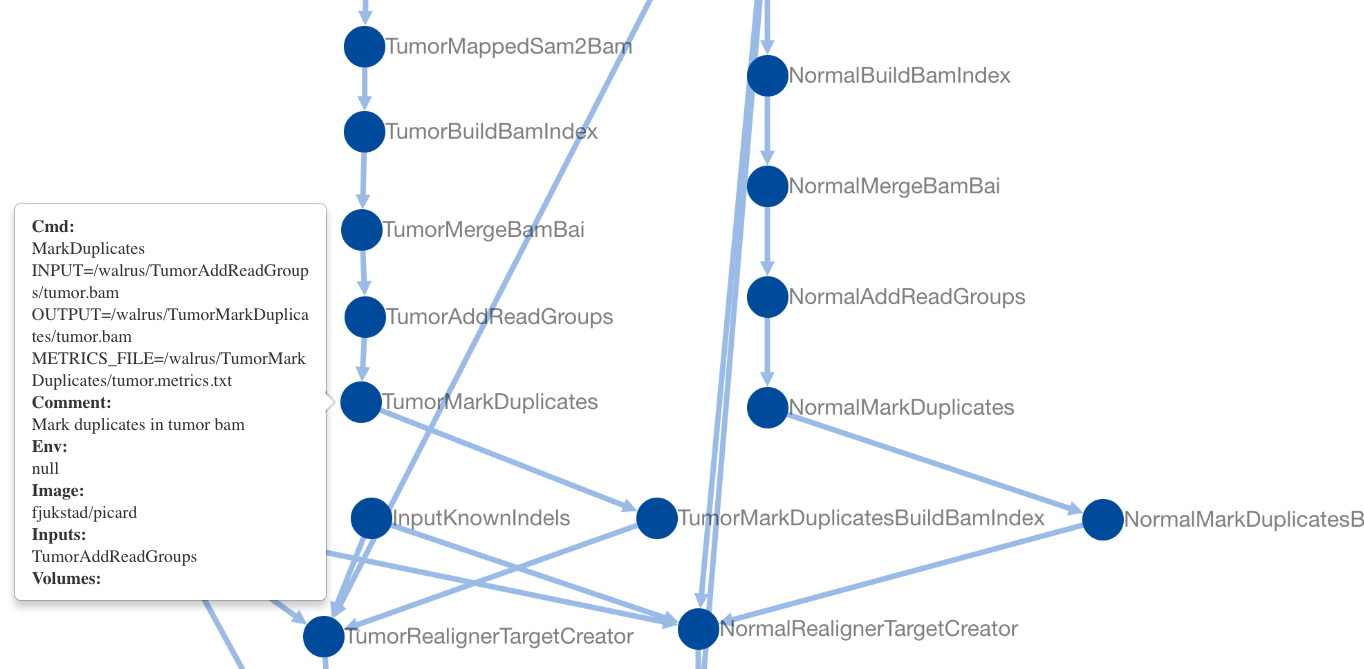
\includegraphics[width=10cm]{figures/webshot.png}
    \caption[Screenshot of the web-based visualization in
    \texttt{walrus}]{Screenshot of the web-based visualization in
    \texttt{walrus}. The user has zoomed in to inspect the pipeline step which
    marks duplicate reads in the tumor sequence data.}
    \label{webshotfig}
\end{figure} 

From the analyses we discovered inherited germline mutations that are recognized
to be among the top 50 mutations associated with an increased risk of familial
breast cancer. We also discovered a germline deletion which has been associated
with an increased risk of breast cancer. We also discovered mutations in a
specific gene that might explain why specific drug had not been effective in the
treatment of the primary tumor. From the profile of the primary tumor we
discovered many somatic events (around 30 000) across the whole genome with
about 1000 in coding regions, and 500 of these were coding for non-synonymous
mutations.  We did not see amplification or constituent activation of growth
factors like HER2, EGFR or other players in breast cancer. Because of the
germline mutation, early recurrence, and lack of DNA events, we suspect that the
patient's primary tumor was highly immunogenic. We have also identified several
mutations and copy number changes in key driver genes. This includes a mutation
in a gene that creates a premature stop codon, truncating one copy of the gene.

While we cannot share the results in details or the sensitive dataset, we have
made the pipeline description available at \url{github.com/uit-bdps/walrus}
along with other example pipelines. 

\subsection{Example Dataset}
To demonstrate the performance of \texttt{walrus} and the ability to track and
detect changes in an analysis pipeline, we have implemented one of the variant
calling pipelines from \cite{cornish2015comparison} using tools from picard and
the \gls{gatk}. We show the storage and computational overhead of our approach,
and the benefit of capturing the pipeline specification using a pipeline
manager.  The pipeline description and code is available along with
\texttt{walrus} at \url{github.com/uit-bdps/walrus}. Figure
\ref{benchpipefigure} shows a simple graphical representation of the pipeline. 

\begin{figure}
    \centering
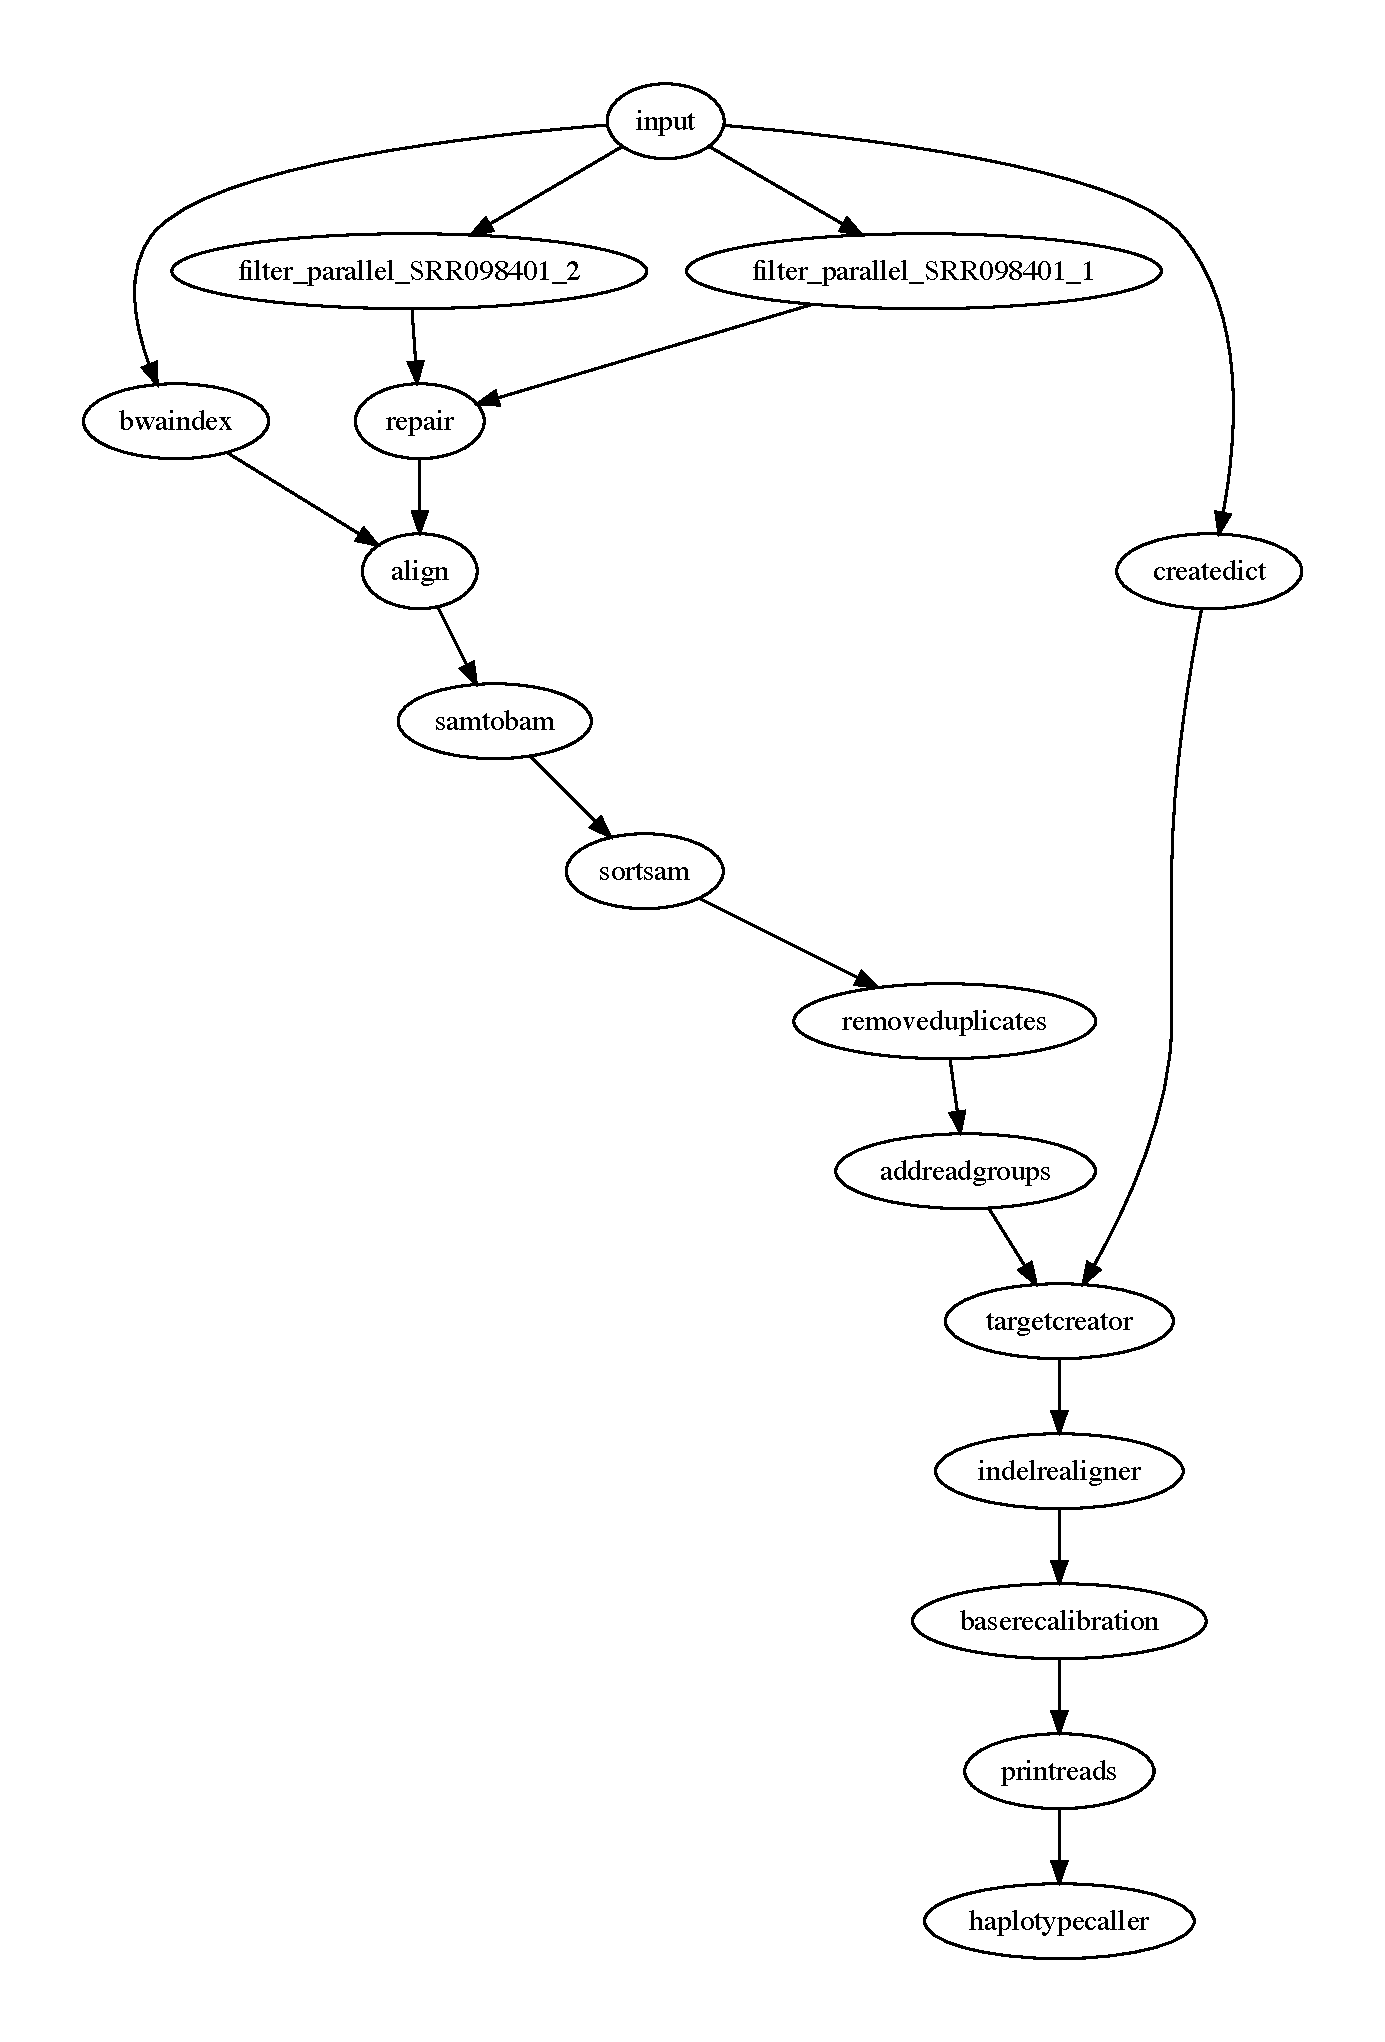
\includegraphics[width=\linewidth]{figures/graph.pdf}
    \caption[DOT representations of a pipeline in \texttt{walrus}]{In addition
    to the web-based inteactive pipeline visualization, \texttt{walrus} can also
    generate DOT representations of pipelines. The figure shows the example
    variant calling pipeline we used in the performance evaluation.} 
    \label{benchpipefigure}
\end{figure} 

\subsection{Performance and Resource Usage}
We first run the variant calling pipeline without any additional provenance
tracking or storing of output or intermediate datasets. This is to get a
baseline performance measurement for how long we expect the pipeline to run. We
then run a second experiment to measure the overhead of versioning output and
intermediate data. Then we introduce a parameter change in one of the pipeline
steps which results in new intermediate and output datasets. Specifically we
change the \texttt{--maxReadsForRealignment} parameter in the indel realigner
step back to its default (See the online pipeline description for more details).
This forces \texttt{walrus} to recompute the indel realigner step and any
subsequent steps.  To illustrate how \texttt{walrus} can restore old pipeline
configurations and results, we restore the pipeline to the initial configuration
and results. We show the computational overhead and storage usage of restoring a
previous pipeline configuration. 

Reproducing results from a scientific publication can be a difficult task. For
example, because the rendering of the online version of the pipeline in
\cite{cornish2015comparison} converts two consecutive hypens (\texttt{--})
into single em dashes (---), the pipeline will not run using the specified input
parameters. However, PDF versions of the paper lists the parameters correctly.
In addition, the input filenames in the variant calling step do not correspond
to any output files in previous steps, but because of their similarity to
previous output files we assume that this is just a typo.  These issues in
addition to missing commands for e.g. the filtering step highlights the clear
benefit of writing and reporting the analysis pipeline using a tool such as
\texttt{walrus}. 

Table \ref{resultstable} shows the runtime and storage use of the different
experiments. In the second experiment we can see the added overhead of adding
version control to the dataset. In total, an hour is added to the runtime and
the data size is doubled. The doubling comes from git-lfs hard copying the data
into a subdirectory of the \texttt{.git} folder in the repository. With git-lfs
users can move all datasets to a remote server reducing the local storage
requirements. 
In the third experiment we can see that only the downstream analyses from
configuring the indel realignment parameter is executed. It generates 30GB of
additional data, but the execution time is limited to the applicable stages.
Restoring the pipeline to a previous configuration is almost instantaneous since
the data is already available locally and git only has to modify the pointers to
the correct files in the \texttt{.git} subdirectory. 

\begin{table}[ht!]
    \centering
    \caption{Runtime and storage use of the example variant-calling pipeline
    developed with \texttt{walrus}.} 
    \begin{tabular}{ | c | p{4cm} | p{2cm} | p{2cm} |}
    \hline
    Experiment & Task & Runtime & Storage Use \\ \hline
    1 & Run pipeline with default configuration & 21 hours 50 minutes & 235 GB
        \\ \hline
    2 & Run the default pipeline with version control of data & 23 hours 9
        minutes & 470 GB \\ \hline
    3 & Re-run the pipeline with modified indel realignment parameter & 13 hours
        & 500 GB \\ \hline
    4 & Restoring pipeline back to the default configuration & < 1 second &
        500GB \\ \hline
%    5 & Examining the pipeline output & TBD & 500GB \\ \hline 
    \end{tabular}
    \label{resultstable}
\end{table}


% \subsubsection{Provenance} 
% Listing \ref{provlist} shows the output of task 5, examining the pipeline output
% against previous versions. It shows how the subsequent pipeline steps have been
% re-run and that the pipeline description was changed. 


\section{Related Work} 
There are a wealth of pipeline specification formats and workflow managers
available. Some are targeted at users with programming experience while others
provide simple \glspl{gui}. 

We have previously conducted a survey of different
specialized bioinformatics pipelines.\cite{fjukstad2017review} 
The pipelines were selected to show how analysis pipelines for different
applications use different technologies for configuring, executing and storing
intermediate and output data. In the review, we targeted specialized analysis
pipelines that support scaling out the pipelines to run on \gls{hpc} or cloud
computing platforms. 

Here we describe general systems for developing data analysis
pipelines, not just specialized bioinformatics pipelines. While most provide
viable options for genomic analyses, we have found most to complex to install
and maintain in clinical settings. We discuss tools that use the common
\gls{cwl} pipeline specification and systems that provide versioning of data. 

\gls{cwl} is a specification for describing analysis workflows and
tools.\cite{cwl} A pipeline is written as a \gls{json} or \gls{yaml} file,
or a mix of the two, and describes each step in detail, e.g. what tool to run,
its input parameters, input data and output data. The pipeline descriptions
are text files that can be under version control and shared between projects. There
are multiple implementations of \gls{cwl} workflow platforms, e.g. the reference
implementation cwl\_runner\cite{cwl}, Arvados\cite{arvados}, Rabix\cite{rabix},
Toil\cite{toil}, Galaxy\cite{goecks2010galaxy}, and AWE.\cite{awe} It is no
requirement to run tools within containers, but implementations can support it.
There are few of these tools that support versioning of the data.  Galaxy is an
open web-based platform for reproducible analysis of large high-throughput
datasets.\cite{goecks2010galaxy} It is possible to run Galaxy on local compute
clusters, in the cloud, or using the online Galaxy site.\footnote{Available at
\url{usegalaxy.org}.} In Galaxy users set up an analysis pipeline using a
web-based graphical interface, and it is also possible to export or import an
existing workflow to an \gls{xml} file.\footnote{An alpha version of Galaxy with
\gls{cwl} support is available at
\url{github.com/common-workflow-language/galaxy}.}  We chose not to use Galaxy
because of missing command-line and scripting support, along with little support
for running workflows with different configurations.\cite{spjuth2015experiences}
Rabix provides checksums of output data to verify it against the actual output
from the pipeline. This is similar to the checksums found in the git-lfs pointer
files, but they do not store the original files for later. An interesting
project that uses CWL in production is The Cancer Genomics
Cloud\cite{lau2017cancer}. They currently support CWL version 1.0 and are
planning on integrating Rabix as its CWL executor. 
Arvados stores the
data in a distributed storage system, Keep, that provides both storage and
versioning of data. We chose not to use \gls{cwl} and its implementations
because of its relaxed restrictions on having to use containers, its verbose
pipeline descriptions, and the complex compute architecture required for some
implementations. We are however experimenting with an extension to
\texttt{walrus} that translates pipeline descriptions written in \texttt{walrus}
to \gls{cwl} pipeline descriptions. 

Pachyderm is a system for running  big data analysis pipelines. It provides
complete version control for data and leverages the container ecosystem to
provide reproducible data processing.\cite{pachyderm} Pachyderm
consists of a file system (\gls{pfs}) and a processing system (\gls{pps}).
\gls{pfs} is a file system with git-like semantics for storing data used
in data analysis pipelines. Pachyderm ensures complete analysis reproducibility
by providing version control for datasets in addition to the containerized
execution environments. Both \gls{pfs} and \gls{pps} is implemented on top
of Kubernetes.\cite{kubernetes} We believe that the approach in
Pachyderm with version controlling datasets and containerizing each pipeline
step is the correct approach to truly reproducible data analysis pipelines. 
The reason we did not use Kubernetes and Pachyderm was because our compute
infrastructure did not support it. In addition, we did not want to use a separate
tool, \gls{pfs}, for data versioning, we wanted to integrate it with our current
pratice of using git for versioning. 

Snakemake is a long-running project for analyzing bioinformatic
datasets.\cite{koster2012snakemake} It uses a Python-based language to describe
pipelines, similar to the familiar Makefile syntax, and can execute these
pipelines on local machines, compute clusters or in the cloud. To ensure
reproducible workflows, Snakemake integrates with Bioconda to provide the
correct versions of the different tools used in the workflows. It integrates
with Docker and Singularity containers\cite{singularity} to provide isolated
execution, and in later versions Snakemake allows pipeline execution on a
Kubernetes cluster. Because Snakemake did not provide necessary integration with
software containers at the time we developing our analysis pipeline, we did not
find it to be a viable alternative. For example, support for pipelines
consisting of Docker containers pre-installed with bioinformatics tools came a
year later than walrus. 

Another alternative to develop analysis pipelines is
Nextflow.\cite{di2017nextflow} Nextflow uses its own language to describe
analysis pipelines and supports execution within Docker and Singularity
containers. 

As discussed in \cite{NIK, fjukstad2017review}, recent projects propose to use
containers for life science research. The BioContainers and
Bioboxes\cite{belmann2015bioboxes} projects address the challenge of installing
bioinformatics data analysis tools by maintaining a repository of Docker
containers for commonly used data analysis tools. Docker containers are shown to
have better than, or equal performance as \glspl{vm}.\cite{di2015impact} Both
forms of virtualization techniques introduce overhead in I/O-intensive
workloads, especially in \glspl{vm}, but introduce negligible CPU and memory
overhead. For precision medicine pipelines the overhead of Docker containers
will be negligible since these tend to be compute-intensive and they typically
run for several hours.\cite{di2015impact} Containers have also been proposed as
a solution to improve experiment reproducibility, by ensuring that the data
analysis tools are installed with the same
responsibilities.\cite{boettiger2015introduction} 

\section{Discussion}
Precision medicine requires flexible analysis pipelines that allow researchers
to explore different tools and parameters to analyze their data.  While there
are best practices to develop analysis pipelines for genomic datasets, e.g. to
discover genomic variants, there is still no de-facto standard for sharing the
detailed descriptions to simplify re-using and reproducing existing work.
Pipelines typically need to be tailored to fit each project and patient, and
different patients will typically elicit different molecular patterns that
require individual investigation. While we could follow the best practices to
develop our pipeline we explored different tools and parameters before we
arrived at the final analysis pipeline.  For example, in our \gls{wes} pipeline
we ran several rounds of preprocessing (trimming reads and quality control)
before we were sure that the data was ready for analysis. Having a pipeline
system that could keep track of different intermediate datasets, along with the
pipeline specification, simplifies the task of comparing the results from
pipeline tools and input parameters. While we have developed one approach to
version control genomic datasets in an analysis pipeline, we believe that there
is still room for improvement. 

While we provide one approach to version control datasets, there are still some
drawbacks. \texttt{git-lfs} supports large files, but in our results it added
5\% in runtime.  This makes the entire analysis pipeline slower, but we argue
that having the files under version control outweigh the runtime. In addition,
there are only a few public \texttt{gif-lfs} hosting platforms for datasets
larger than a few gigabytes, making it necessary to host these in-house.
In-house hosting may also be a requirement at different medical institutions.  

We aim to investigate the performance of running analysis pipelines with
\texttt{walrus}, and the potential benefit of its built-in data parallelism.
While our \gls{wes} analysis pipeline successfully run steps in parallel for the
tumor and adjacent normal tissue, we have not demonstrated the benefit
of doing so. This includes benchmarking and analyzing the system requirements
for doing precision medicine analyses.  We are also planning on exploring
parallelism strategies where we can split an input dataset into chromosomes and
run some steps in parallel for each chromosome, before merging the data again. 

We believe that future data analysis systems for precision medicine will follow
the lines of our proposed approach. Software container solutions provide
valuable information in the reporting of the analyses, and they impose little
performance overhead. Further, the development of container orchestration
systems such as Kubernetes is getting wide adoption nowadays, especially in
web-scale internet companies. However, the adoption of such systems in a
clinical setting depend on support from more tools, and also the addition
of new compute infrastructure. 

\section{Conclusions} 
We have designed and implemented \texttt{walrus}, a tool for developing 
reproducible data analysis pipelines for use in precision medicine. Precision
medicine requires that analyses are run on hospital compute infrastructures and
results are fully reproducible. By packaging analysis tools in software
containers, and tracking both intermediate and output data, \texttt{walrus}
provides the foundation for reproducible data analyses in the clinical setting.
We have used \texttt{walrus} to analyze a patient's metastatic lesions and
adjacent normal tissue to provide insights and recommendations for  cancer
treatment. 

\chapter{Conclusion}
How should we design systems for analyzing and exploring the high-throughput
datasets that facilitate sharing, reuse, and reproducibility? This dissertation
shows that in many cases the solution is to decompose the applications into
small entities that communicate using open protocols. This enables the
development of unified systems for reproducible exploration and analysis. 

While high-throughput datasets and computing systems will undoubtedly evolve, we
believe that the \gls{sme} approach proposed here can offer a new perspective on
developing applications for exploring and analyzing biological data. We hope
that our approach can steer the development of bioinformatics applications away
from large monolithic applications to applications composed of diverse systems.
We believe that this approach can help the community develop new systems to
faster meet the needs of the upcoming biological dataset analyses. 

In Chapter \ref{biodata} we show an approach to store the biological data and
analysis code from a complex epidemiological study in a shareable software
package. We show how we explicitly track versions of code and data, and how we
can generate reproducible data analysis reports for the processed datasets.
We believe that future studies can benefit from applying our approach, and that
future advances in research is dependent on sharing of both datasets and
analysis code. 
% We also show the usefulness our approach as a basis for standardizing the
% preprocessing of its biological datasets. 
In chapter \ref{interactive} we show how we can build
interactive data exploration applications that interface with these software
packages through a microservice architecture. We have implemented this approach
through the microservices in \emph{Kvik}. We show that this architecture style
is suitable for building such applications, and have used it to develop the
\emph{Kvik Pathways} and \emph{MIxT} web applications. These have been
successfully used to explore transcriptional profiles in the \gls{nowac} study,
especially to investigate the interactions between genes and pathways in the
patient tumor and blood cells. 
We believe that the research community in general will benefit greatly if more
projects start to develop their applications using our approach. It simplifies
sharing of computational resources, and we believe that the future of research
will depend on collaborative efforts. 
In chapter \ref{pipeline} use the same approach, to compose systems of disparate
tools, for developing biological data
analysis pipelines, implemented in \texttt{walrus}. 
To ensure reproducible results, we supplement the processing
with data versioning to track provenance of the data through the pipeline and
across pipeline versions. We have used \texttt{walrus} in the clinical setting
to develop a \gls{wes} pipeline for discovering \glspl{snp}, genomic
variants, and somatic mutations, in a breast cancer patient's metastatic
lesion. 

Combined, these systems demonstrate the applicability of our approach across a
range of different use cases. 

In the rest of this chapter we summarize end-to-end lessons learned during this
work. We then discuss the work in the context of research and in the clinical
setting,
before we propose areas for future work. 


\section{Lessons Learned}
Through the design of the \gls{sme} approach for analyzing and exploring
biological datasets, as well as the different implementations of the approach,
we have solved challenges and learned some key lessons.

\textbf{There is no single solution programming language or system.} 
In the field of bioinformatics there have been tremendous efforts to develop
analysis tools for improving the analysis of new biological datasets.  This has
led to systems being written in a plethora of different languages, and deployed
on top of different systems. This is the main motivation behind our \gls{sme}
approach together with software containers.

\textbf{Take advantage of existing tools.} The ability to develop applications
for analyzing biological datasets comes from the availability of existing tools.
By developing easy-to-use interfaces for the existing tools, it is possible
to develop new applications without reimplementing key features. 

\textbf{Simplicity is key.} When proposing a new approach for either managing
datasets, writing data exploration applications, or developing analysis
pipelines, it is not possible to overstate the importance of the simplicity of
the solution. 

\textbf{Researchers are not software engineers.} 
When designing a new approach to store and analyze high-throughout biological
datasets, it is important to remember that its users have limited software
engineering backgrounds. Especially when the implementation is based on complex
systems such as \texttt{git}, the learning curve for the system is steep and
require training of its users. In our project we have organized workshops in
both R and git to get the researchers in the \gls{nowac} study comfortable with
these systems to follow our best practices. 

% \textbf{Define the data storage and analysis requirements before collecting
% data.} 

% \section{Broader Impact}
% balkanized 
% clinica

\section{Future Work}
As we have discussed in previous chapters, there are some limitations to our
approach and its implementations. To summarize these, the main areas for
improvement are: 

\begin{itemize} 

\item \textbf{Versioning of datasets:} \texttt{git} was not designed to version
large binary files, such as biological datasets, and it does not provide the
required performance or scalability to version the large biological data. 

% Rob Pike said this: 
% Measure. Don't tune for speed until you've measured, and even then don't
% unless one part of the code overwhelms the rest.
% http://www.catb.org/~esr/writings/taoup/html/ch01s06.html
\item \textbf{Additional evaluation:} while we have shown that the \gls{sme}
approach can be used to develop systems for managing research data, developing
interactive applications and data analysis pipelines, we would like to
better understand its performance and scalability. 

\item \textbf{Refactoring and test coverage:} while we provide fully implemented
solutions for data storage, interactive applications, and data analysis
pipelines, they all have areas of improvement with regards to performance,
scalability, and robustness. 

\item \textbf{Distributed execution:} while \texttt{walrus} orchestrate
execution of Docker containers, we do not support the execution of these on
multiple compute nodes. Distributing the computation on multiple machines will
reduce the execution time if we can share the data across the
machines efficiently. We would also like to evaluate the possibility of using an
existing container orchestration system, such as
Kubernetes, to orchestrate the execution of an analysis pipeline. Many of these
already provide functionality for distributed execution of software containers. 

\item \textbf{Wide adoption of a pipeline description format:} we are not the
first to propose a new computing standard.\footnote{\url{xkcd.com/927}} We found
that the current standards were either too verbose, e.g., \gls{cwl}, or did not
enforce the use of software containers. This led us to our own description
format, but we recognize the need for a single open standard, and hope to
contribute to its development. 

\end{itemize} 

We aim to refine and continue development on our \glspl{sme} approach to address
these challenges, and that we can inspire a more unified development community
in bioinformatics. We believe that the future of cancer research relies on the
successful integration of diverse data analysis and storage systems from
different research institutions.  This will definitely continue to be an
interesting area of research.


 

\backmatter

\bibliographystyle{IEEEtran}
\bibliography{references}

\appendix
\begin{appendix}
    \chapter{Paper 1} 
    \bibentry{fjukstad2015kvik} \\~\\
    \emph{ The following includes 5 of the 15 total pages. The first 5 pages is
    the paper, while remaining 10 pages are open reviews, responses, and
    additions to the final version of the paper. These are available online at
    \url{f1000research.com/articles/4-81/v2}}
    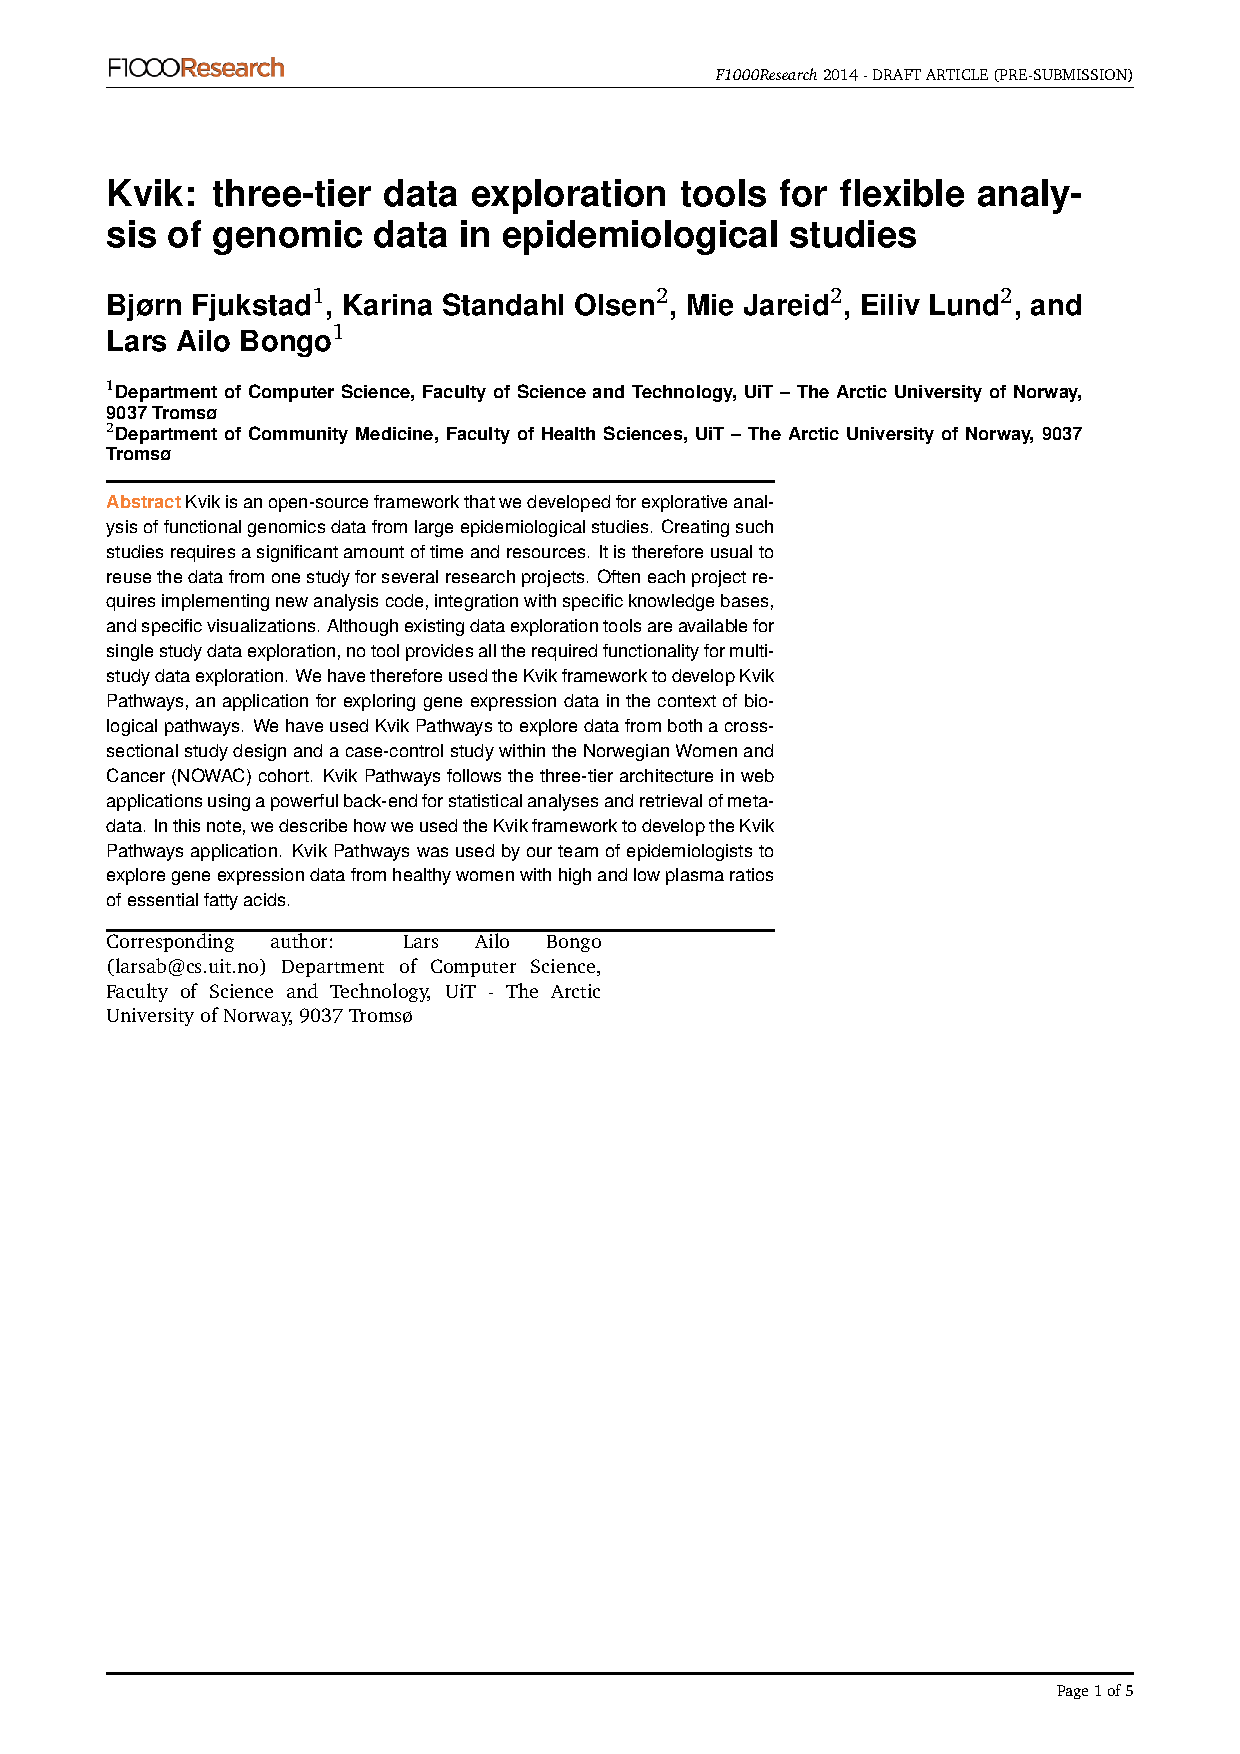
\includepdf[pages={1-5}]{papers/fjukstad2015kvik.pdf}
    \newpage
    
    \chapter{Paper 2} 
    \bibentry{fjukstad2017building}
    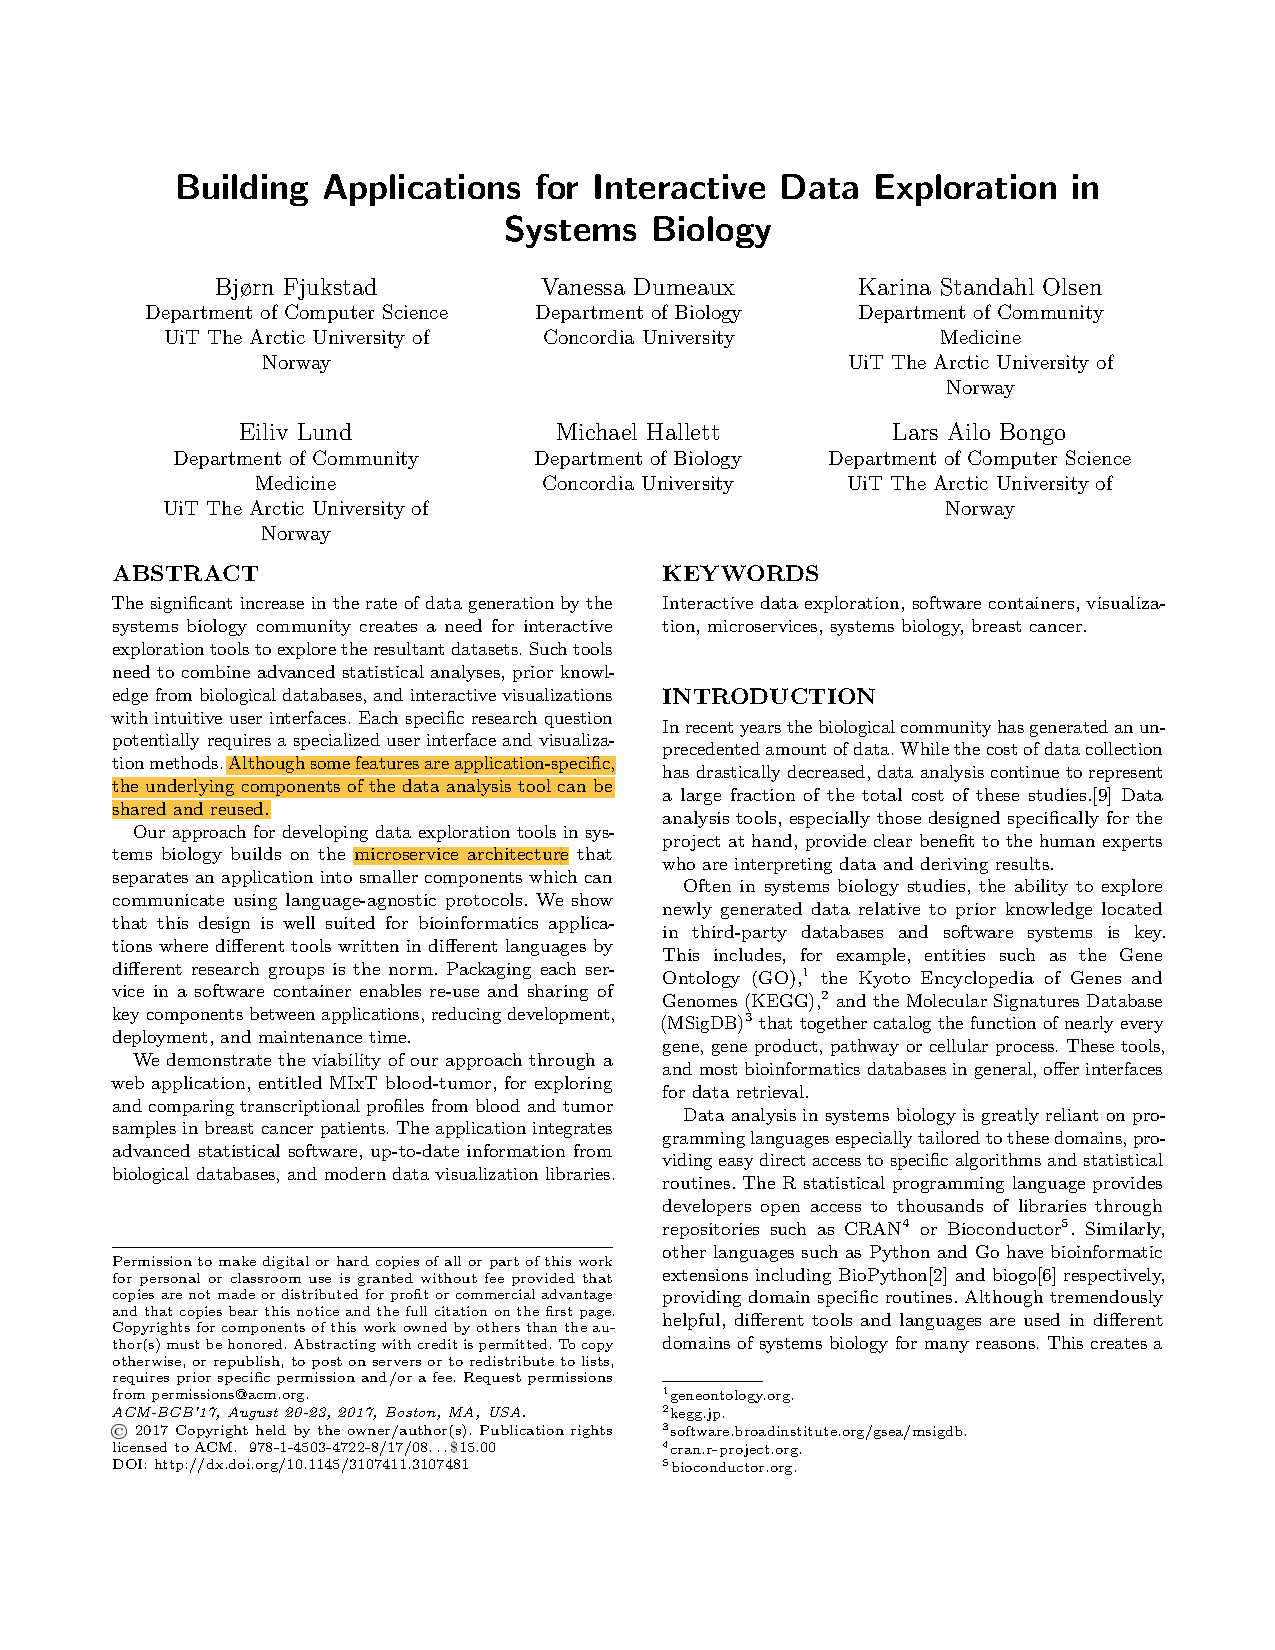
\includepdf[pages={1-6}]{papers/fjukstad2017building.pdf}

    \chapter{Paper 3} 
    \bibentry{dumeaux2017interactions}
    \includepdf[pages={1-27}]{papers/dumeaux2017interactions.pdf}

    \chapter{Paper 4} 
    \bibentry{fjukstad2017review}
    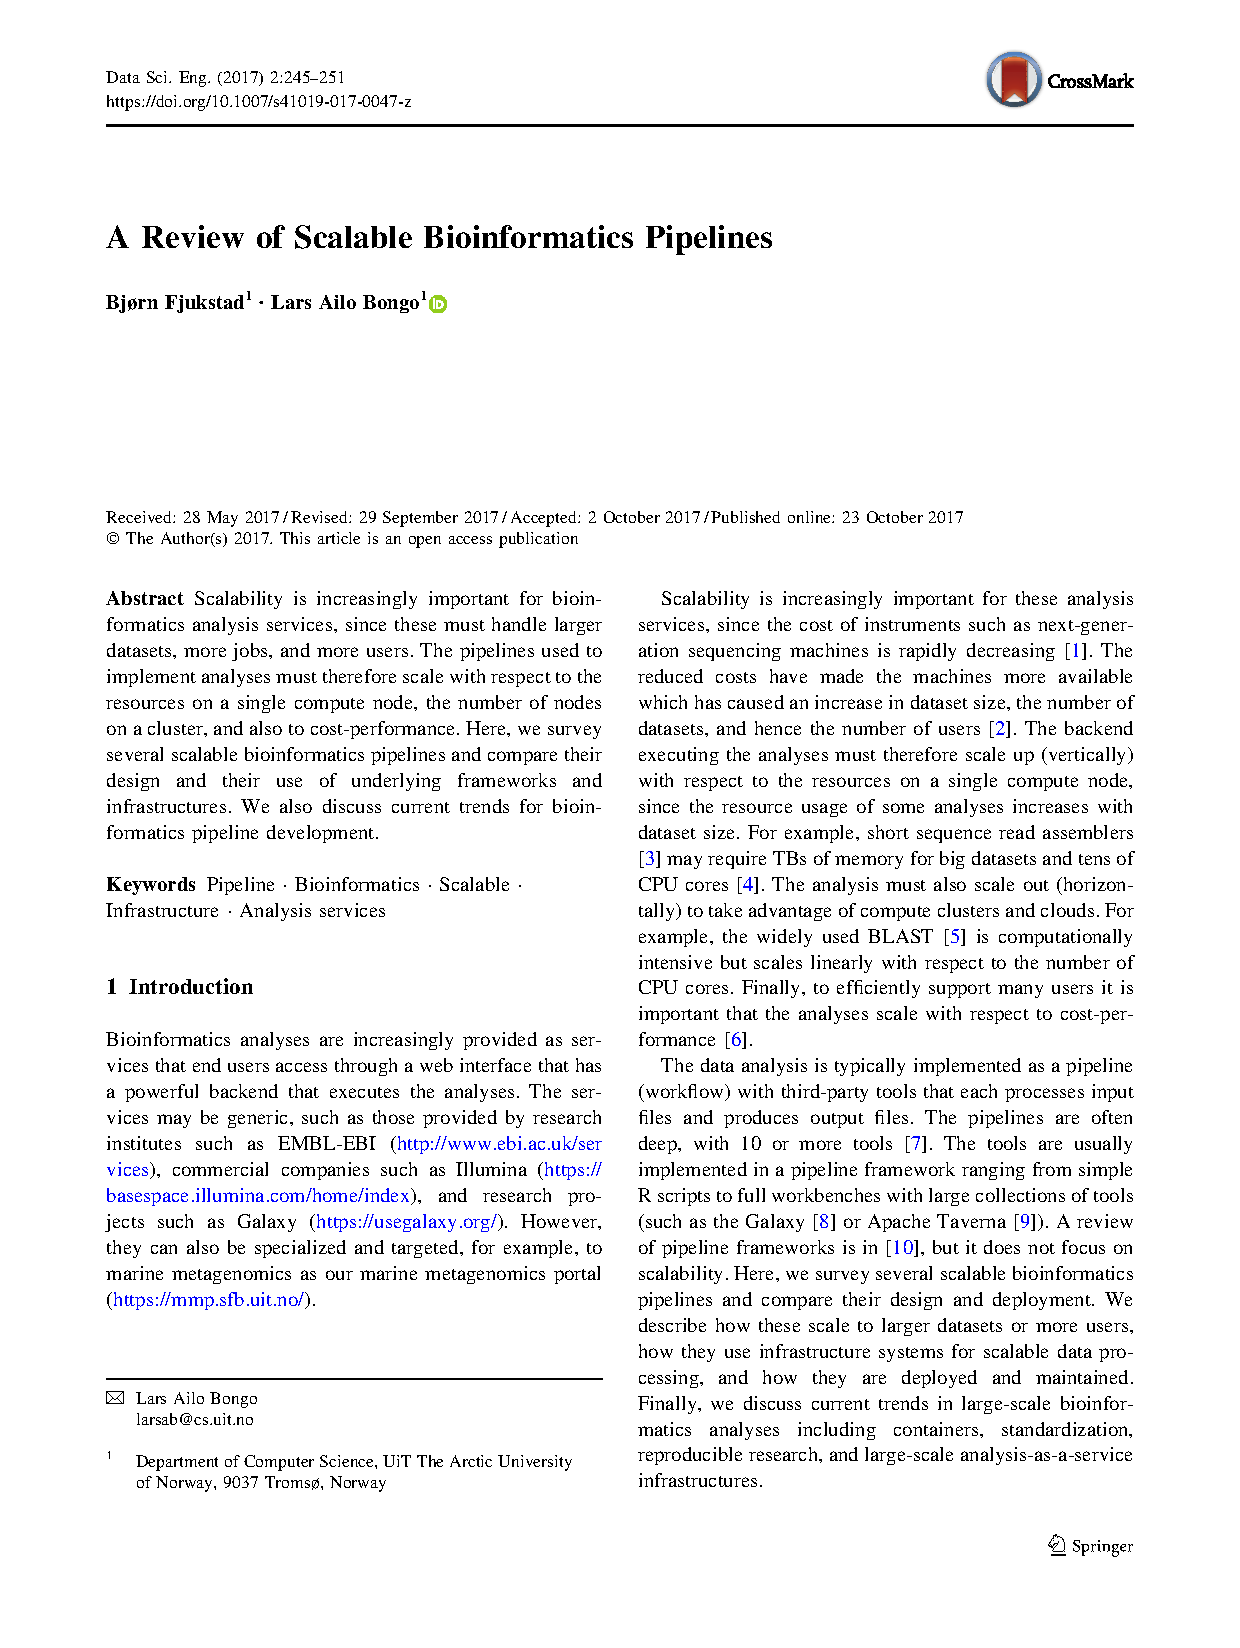
\includepdf[pages={1-7}]{papers/fjukstad2017review.pdf}

    \chapter{Paper 5} 
    \bibentry{NIK}
    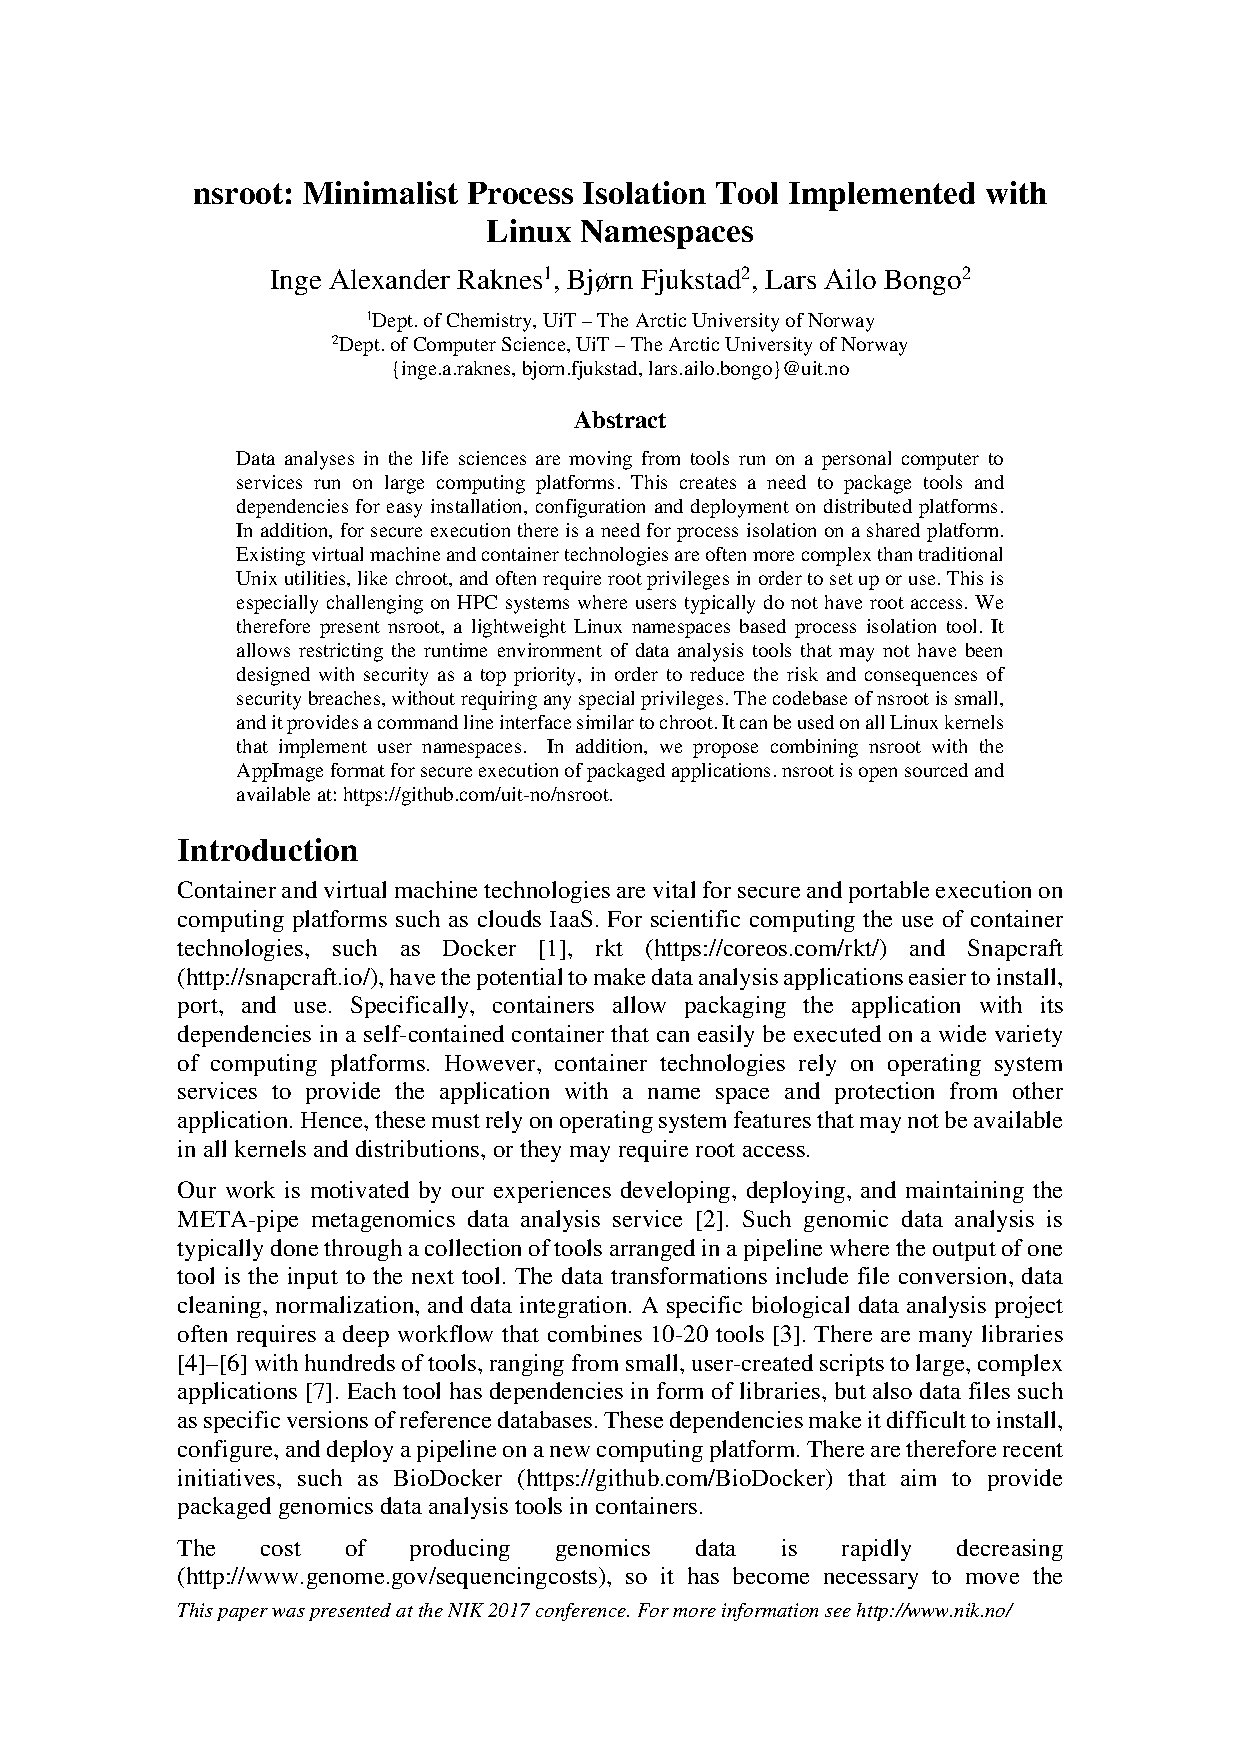
\includepdf[pages={1-6}]{papers/NIK.pdf}

    \chapter{Paper 6} 
    \bibentry{walrus}
    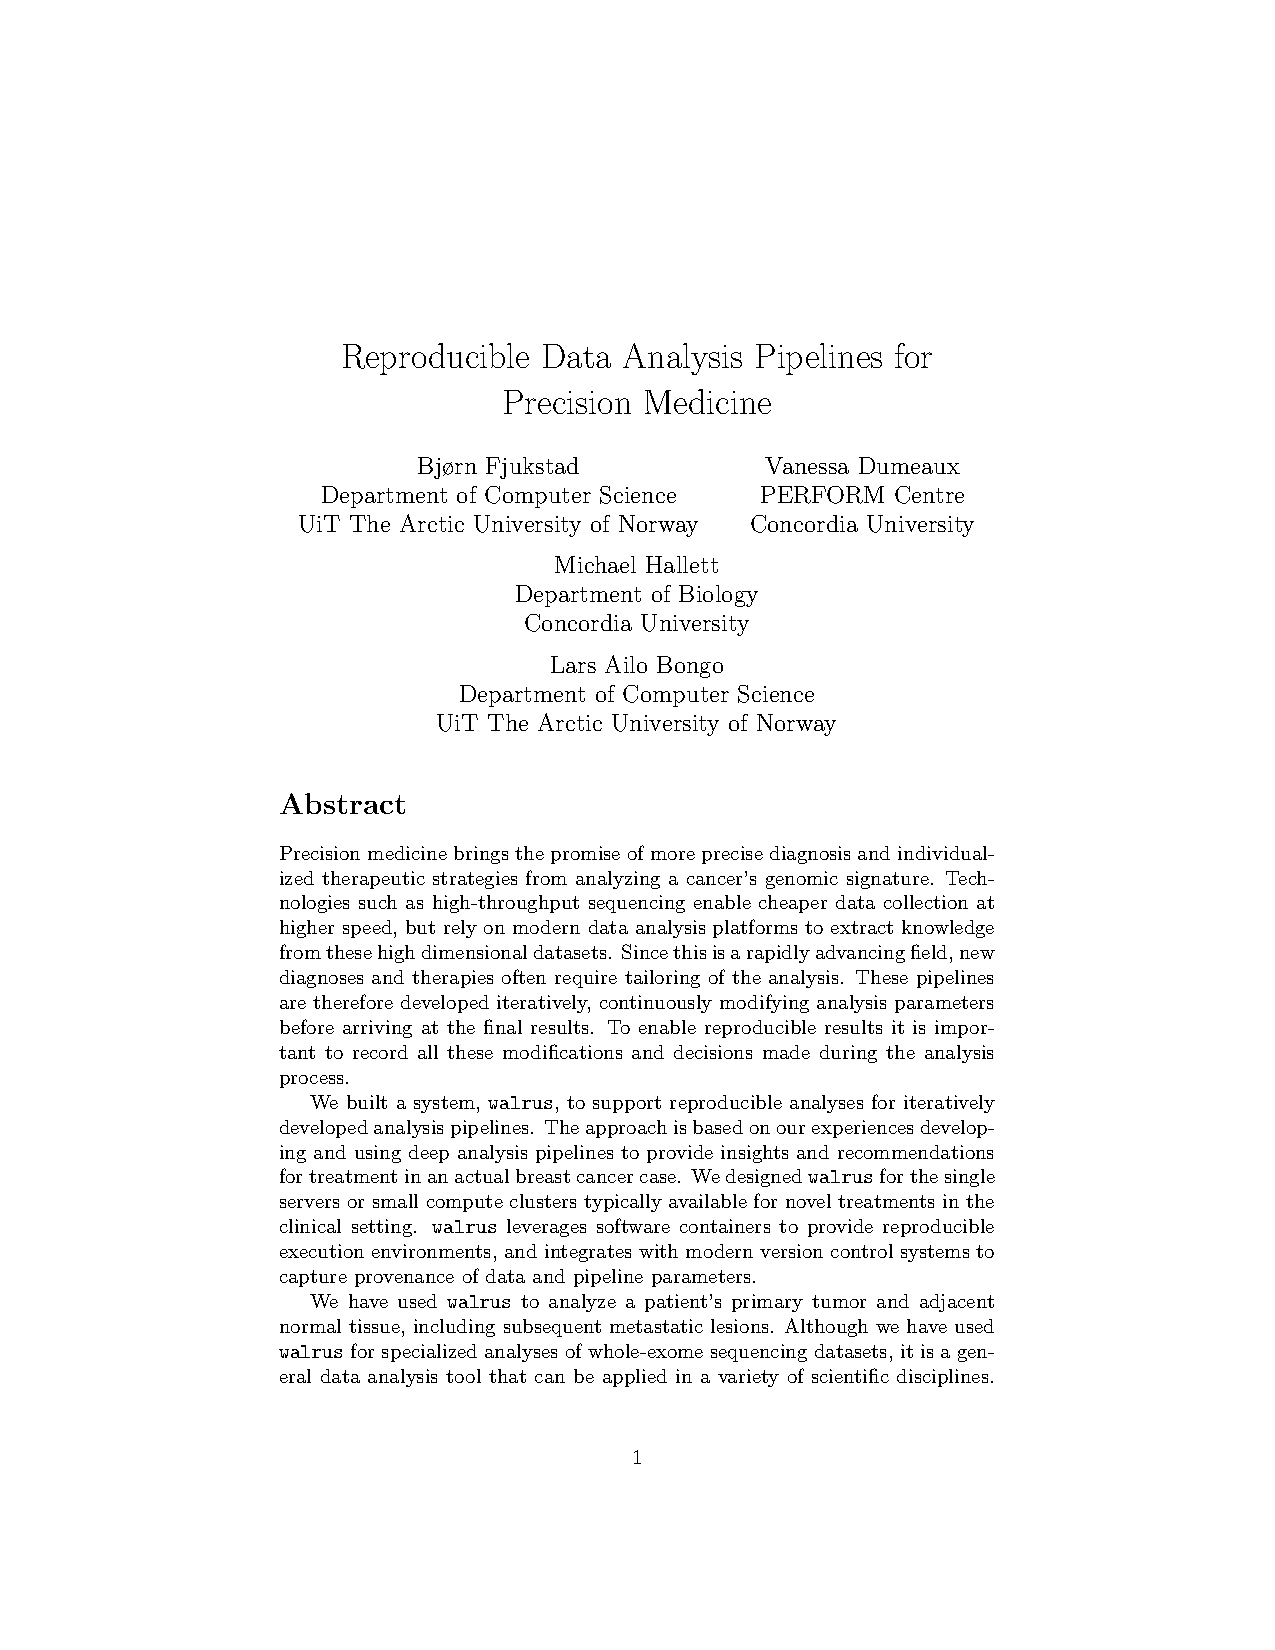
\includepdf[pages={1-16}]{papers/walrus.pdf}
\end{appendix}
\end{document} 
